% !TEX program = pdflatex

\documentclass[aspectratio=169]{beamer}

% -------------------------------------------------
% Codificação e idioma (pdflatex puro)
% -------------------------------------------------
\usepackage[utf8]{inputenc}
\usepackage[T1]{fontenc}
\usepackage[brazilian]{babel}
\usepackage{lmodern}

% -------------------------------------------------
% Pacotes permitidos / necessários
% -------------------------------------------------
\usepackage{graphicx}
\usepackage{tikz}
\usetikzlibrary{positioning, arrows.meta, shapes.geometric, calc}
\usepackage{xcolor}
\usepackage{hyperref}
\usepackage[most]{tcolorbox}
\usepackage{fontawesome5}
\usepackage{amsmath}
\usepackage{amssymb}
\usepackage{booktabs}
\usepackage{etoolbox}
\usepackage{listings}

% -------------------------------------------------
% Tema visual base + paleta UFABC
% -------------------------------------------------
\usetheme{Madrid}
\definecolor{UFABCGreen}{HTML}{006633}
\definecolor{UFABCYellow}{HTML}{FFD500}
\definecolor{UFABCLightGreen}{HTML}{E8F3EC}
\definecolor{UFABCLightYellow}{HTML}{FFF6CC}
\definecolor{SoftGray}{HTML}{F3F4F6}

\setbeamercolor{title}{fg=white,bg=UFABCGreen}
\setbeamercolor{frametitle}{fg=white,bg=UFABCGreen}
\setbeamercolor{structure}{fg=UFABCGreen}
\setbeamercolor{normal text}{fg=black,bg=white}
\setbeamercolor{item}{fg=UFABCGreen}
\setbeamercolor{section in head/foot}{bg=UFABCGreen,fg=white}
\setbeamercolor{subsection in head/foot}{bg=UFABCGreen,fg=white}
\setbeamerfont{frametitle}{size=\normalsize,series=\bfseries}
\setbeamertemplate{navigation symbols}{}

\setbeamertemplate{headline}{%
  \begin{beamercolorbox}[wd=\paperwidth,ht=7ex,dp=1.2ex,leftskip=0.5cm]{section in head/foot}%
    \vbox to 7ex{%
      \vfil
      \hbox{
\includegraphics[height=0.85cm]{logo_ufabc.png}}%
      \vfil
    }%
  \end{beamercolorbox}%
}

\AtBeginEnvironment{frame}{\small}

% -------------------------------------------------
% Metadados
% -------------------------------------------------
\title[EITduino --- Interface PyQt para TIE]{Desenvolvimento de Interface PyQt para Controle de Parâmetros em Tomografia por Impedância Elétrica usando pyEIT}
\author[Lucas Maio Nunes de Almeida Gonçalves]{Lucas Maio Nunes de Almeida Gonçalves}
\institute[UFABC]{Universidade Federal do ABC --- Engenharia Biomédica\\[0.2em]\textbf{Orientador:} Prof. Dr. Erick Dario Leon Bueno de Camargo}
\date{2026}

% -------------------------------------------------
% Estilos auxiliares
% -------------------------------------------------
\tcbset{
  ufabcbox/.style={
    enhanced,
    colback=UFABCLightGreen,
    colframe=UFABCGreen,
    boxrule=0.9pt,
    sharp corners,
    title filled,
    colbacktitle=UFABCGreen,
    coltitle=white,
    fonttitle=\bfseries,
    left=1mm,right=1mm,top=1mm,bottom=1mm
  },
  ufabcnote/.style={
    enhanced,
    colback=UFABCLightYellow,
    colframe=UFABCYellow!60!black,
    boxrule=0.8pt,
    sharp corners,
    fonttitle=\bfseries,
    colbacktitle=UFABCYellow!75!black,
    coltitle=black,
    left=1mm,right=1mm,top=1mm,bottom=1mm
  }
}

\lstset{
  basicstyle=\ttfamily\scriptsize,
  keywordstyle=\color{UFABCGreen}\bfseries,
  commentstyle=\color{gray!80!black},
  stringstyle=\color{orange!50!black},
  showstringspaces=false,
  frame=single,
  rulecolor=\color{UFABCGreen},
  breaklines=true,
  columns=fullflexible
}

\newcommand{\highlightterm}[1]{\textcolor{UFABCGreen}{\textbf{#1}}}
\newcommand{\accentterm}[1]{\textcolor{UFABCYellow!60!black}{\textbf{#1}}}

\begin{document}

% BLOCO 0 --- Capa e agenda --- alvo: 2 min (~2 slides)
\begin{frame}
\centering
\vspace{0.2cm}
{\Large\bfseries Desenvolvimento de Interface PyQt para Controle de Parâmetros em Tomografia por Impedância Elétrica usando pyEIT\par}
\vspace{1.0cm}

\includegraphics[width=0.30\textwidth]{logo_ufabc.png}\\[1.0cm]
{\normalsize Lucas Maio Nunes de Almeida Gonçalves\par}
\vspace{0.2cm}
{\normalsize Universidade Federal do ABC --- Engenharia Biomédica\par}
\vspace{0.2cm}
{\normalsize Orientador: Prof. Dr. Erick Dario Leon Bueno de Camargo\par}
\vfill
{\small São Bernardo do Campo, SP --- 2026\par}
\end{frame}

\begin{frame}{Agenda}
\begin{tcolorbox}[ufabcbox,title=Roteiro da apresentação]
\begin{itemize}
  \item Contexto e motivação
  \item Fundamentação teórica
  \item Metodologia
  \item Resultados
  \item Demo e conclusão
\end{itemize}
\end{tcolorbox}
\end{frame}

% BLOCO 1 --- Contexto: TIE --- alvo: 5 min (~2 slides)
\section{Contexto e motivação}

% BLOCO 2 --- Motivação e objetivos --- alvo: 5 min (~3 slides)
\begin{frame}{Motivação}
\begin{tcolorbox}[ufabcbox,title=Problema prático]
\begin{itemize}
  \item \texttt{pyEIT} é uma biblioteca open-source madura para reconstrução em TIE, mas é uma biblioteca, não uma ferramenta interativa.
  \item Há um \textbf{gap} de interface voltada a ensino e pesquisa que permita explorar comparativamente o efeito de métodos e parâmetros.
\end{itemize}
\end{tcolorbox}
\end{frame}

\begin{frame}{Objetivos específicos}
\vspace{-0.6em}
\begin{tcolorbox}[ufabcbox,title=Objetivos específicos]
\footnotesize
\begin{enumerate}\setlength{\itemsep}{2pt}\setlength{\parskip}{0pt}\setlength{\topsep}{2pt}
  \item Estruturar a aplicação inspirado no padrão MVC, desacoplando a reconstrução numérica das interfaces gráficas e implementando um ponto de entrada unificado para seleção do backend.
  \item Implementar e disponibilizar os três métodos do pyEIT --- Back-Projection (BP), Jacobiano (JAC) e GREIT --- permitindo ao usuário compará-los quanto à imagem reconstruída, estabilidade temporal e sensibilidade a ruído.
  \item Realizar uma revisão teórica dos fundamentos da Tomografia por Impedância Elétrica, abrangendo o princípio de medição, os problemas direto e inverso, a abordagem por diferença temporal e os métodos de reconstrução utilizados.
  \item Disponibilizar exploração interativa de parâmetros como densidade da malha, formato geométrico, resolução da grade de renderização e regularização, evidenciando seu impacto na imagem obtida.
  \item Desenvolver uma segunda implementação da interface com PyQtGraph como backend de renderização, permitindo compará-la qualitativamente com a interface principal em organização visual e fluidez.
  \item Organizar o código-fonte de forma modular, favorecendo sua disponibilização, reutilização e extensão em trabalhos futuros.
\end{enumerate}
\end{tcolorbox}
\end{frame}

% BLOCO 3 --- Fundamentação teórica --- alvo: 12 min (~5 slides)
\section{Fundamentação teórica}

\begin{frame}{Problema direto}
\begin{tcolorbox}[ufabcbox,title=Formulação]
\footnotesize
\begin{itemize}\setlength{\itemsep}{2pt}\setlength{\parskip}{0pt}\setlength{\topsep}{2pt}
  \item Dada uma distribuição de condutividade $\sigma(x,y)$ no domínio, calcular as tensões que seriam medidas na fronteira.
  \item Formulação por EDP:
  \[
  \nabla \cdot (\sigma \nabla u) = 0
  \]
  \item Solução numérica por FEM sobre malha triangular.
  \item O \texttt{pyEIT} implementa o solver direto por FEM.
\end{itemize}
\end{tcolorbox}

% FONTE: [21] pyEIT docs + capítulo 3 da tese
\end{frame}

\begin{frame}{Problema inverso e caráter mal-posto}
\begin{tcolorbox}[ufabcbox,title=Reconstrução interna a partir de medidas de fronteira]
\begin{itemize}
  \item A partir das tensões medidas, estimar $\sigma(x,y)$ internamente.
  \item Problema \highlightterm{mal-posto no sentido de Hadamard}: a solução pode não ser única, pode não existir para dados ruidosos, e pequenas perturbações nas medidas podem produzir grandes variações na solução reconstruída.
  \item Condição mais criticamente violada na prática: \textbf{estabilidade}.
  \item Consequência direta: necessidade de regularização.
  \item Abordagem adotada: reconstrução por diferença temporal — reconstrói-se $\Delta\sigma$ entre frame atual e frame de referência; o método \texttt{setVref} armazena o primeiro frame como referência.
\end{itemize}
\end{tcolorbox}

% FONTE: capítulo 3 da tese
\end{frame}

\begin{frame}{Regularização e o parâmetro $\lambda$}
\begin{tcolorbox}[ufabcbox,title=Por que regularizar?]
\footnotesize
\begin{itemize}\setlength{\itemsep}{2pt}\setlength{\parskip}{0pt}\setlength{\topsep}{2pt}
  \item Motivação: estabilizar a solução do problema mal-posto.
  \item Formulação de Tikhonov:
  \[
  \min_x \; \lVert Ax - b \rVert^2 + \lambda \lVert Lx \rVert^2
  \]
  \item Solução analítica implementada pelo \texttt{pyEIT}:
  \[
  \Delta\sigma = (J^\top J + \lambda R)^{-1} J^\top \Delta v
  \]
  \item $\lambda$ pequeno $\rightarrow$ maior sensibilidade a ruído.
  \item $\lambda$ grande $\rightarrow$ super-suavização e perda de contraste.
  \item Tipos de regularização no JAC: \texttt{kotre} e \texttt{lm}.
\end{itemize}
\end{tcolorbox}
\end{frame}

\begin{frame}{Back-Projection (BP)}
\begin{tcolorbox}[ufabcbox,title=Back-Projection (BP)]
\footnotesize
\begin{itemize}\setlength{\itemsep}{3pt}\setlength{\parskip}{0pt}\setlength{\topsep}{2pt}
  \item \textbf{Princípio:} retroprojeção ponderada pela Jacobiana, sem inversão explícita da matriz.
  \item \textbf{Saída:} malha triangular, com necessidade de rasterização para exibição em grade regular.
  \item \textbf{Parâmetro-chave:} suavização temporal $\alpha$:
  \[
  \hat{\sigma}_k = \alpha \cdot \hat{\sigma}_{k-1} + (1-\alpha)\cdot \sigma_k
  \]
  \item \textbf{Observação:} nos resultados obtidos, é o método com menor definição espacial e maior presença de artefatos entre os três --- contrapartida da ausência de inversão regularizada.
\end{itemize}
\end{tcolorbox}
\end{frame}

\begin{frame}{Jacobiano (JAC)}
\begin{tcolorbox}[ufabcbox,title=Jacobiano (JAC)]
\footnotesize
\begin{itemize}\setlength{\itemsep}{3pt}\setlength{\parskip}{0pt}\setlength{\topsep}{2pt}
  \item \textbf{Princípio:} inversão regularizada da Jacobiana.
  \item \textbf{Saída:} malha triangular, com necessidade de rasterização para exibição em grade regular.
  \item \textbf{Parâmetro-chave:} $\lambda$, com regularização \texttt{kotre} ou \texttt{LM}.
  \item \textbf{Observação:} nos resultados obtidos, apresentou maior definição espacial que o BP; o resultado depende significativamente da escolha de $\lambda$, como evidenciado nos slides de resultados.
\end{itemize}
\end{tcolorbox}
\end{frame}

\begin{frame}{GREIT}
\begin{tcolorbox}[ufabcbox,title=GREIT]
\footnotesize
\begin{itemize}\setlength{\itemsep}{3pt}\setlength{\parskip}{0pt}\setlength{\topsep}{2pt}
  \item \textbf{Princípio:} filtragem espacial estatística com matriz de reconstrução pré-computada.
  \item \textbf{Saída:} grade regular 2D.
  \item \textbf{Parâmetro-chave:} $\lambda$.
  \item \textbf{Observação:} nos resultados obtidos, apresentou menor variação visual entre frames consecutivos que o BP e aparência mais suave que o JAC com $\lambda$ baixo; bordas retangulares visíveis são consequência da grade regular.
\end{itemize}
\end{tcolorbox}
\end{frame}

% BLOCO 4 --- Metodologia: arquitetura e dados --- alvo: 12 min (~5 slides)
\section{Metodologia}

\begin{frame}{Dados experimentais}
\begin{columns}[T,totalwidth=\textwidth]
\column{0.56\textwidth}
\begin{tcolorbox}[ufabcbox,title=Conjunto de dados utilizado]
\begin{itemize}
  \item \textbf{Arranjo experimental:} bacia de água (meio condutivo homogêneo) + 8 eletrodos igualmente espaçados + haste sólida como anomalia interna.
  \item 119 frames adquiridos sequencialmente; posição da haste varia no tempo.
  \item Medições \textit{single-ended} (potencial relativo a um eletrodo de referência comum).
  \item Dados fornecidos pelo orientador Prof. Erick Leon.
\end{itemize}
\end{tcolorbox}
% FONTE: seção 4.1 da tese

\column{0.38\textwidth}
\begin{tcolorbox}[ufabcnote,title=Esquema do arranjo experimental]
\centering
\begin{tikzpicture}[scale=0.68]
  % Bacia
  \draw[thick, fill=blue!8] (0,0) circle (2cm);

  % 8 eletrodos
  \foreach \i in {0,...,7} {
    \pgfmathsetmacro{\angle}{90 - \i*45}
    \filldraw[fill=UFABCGreen, draw=black] (\angle:2cm) circle (2.6pt);
    \node[font=\tiny] at (\angle:2.42cm) {E\i};
  }

  % Haste
  \filldraw[fill=gray!60, draw=black] (0.45,0.35) circle (0.18cm);
  \node[font=\scriptsize, text=UFABCGreen] at (0.45,0.72) {haste};

  % Injeção de corrente
  \draw[-{Latex[length=2mm]}, thick, red!70!black]
    (82:2.55cm) arc[start angle=82,end angle=50,radius=2.55cm];
  \node[font=\tiny, text=red!70!black] at (66:2.9cm) {$I$};

  % Legenda
  \node[font=\scriptsize] at (0,-2.75cm) {bacia com água};
\end{tikzpicture}
\end{tcolorbox}
\end{columns}
\end{frame}

\begin{frame}{Arquitetura inspirada em MVC}
\begin{tcolorbox}[ufabcbox,title=Ideia central]
\small Estrutura inspirada no padrão \textit{Model--View--Controller}, com separação entre camada de reconstrução numérica e camada de apresentação.
\end{tcolorbox}

\vspace{0.15cm}
\centering
\begin{tikzpicture}[
  arr/.style={-{Latex[length=2mm]}, thick},
  main/.style={rectangle, rounded corners=2pt, draw=black, fill=gray!20,
               align=center, font=\scriptsize, inner sep=5pt,
               minimum width=5.0cm, minimum height=0.7cm},
  view/.style={rectangle, rounded corners=2pt, draw=black, fill=green!12,
               align=center, font=\scriptsize, inner sep=4pt,
               minimum width=3.8cm, minimum height=0.85cm},
  model/.style={rectangle, rounded corners=2pt, draw=black, fill=yellow!25,
                align=center, font=\scriptsize, inner sep=5pt,
                minimum width=5.0cm, minimum height=0.7cm},
  ext/.style={rectangle, rounded corners=2pt, draw=black, fill=blue!10,
              align=center, font=\scriptsize, inner sep=5pt,
              minimum width=10.5cm, minimum height=0.7cm},
  note/.style={rectangle, draw=UFABCGreen, dashed, rounded corners=2pt,
               fill=white, align=center, font=\tiny, inner sep=3pt,
               text width=3.1cm}
]
\node[main]  (main)  at (0, 0)       {\texttt{main.py} \\ ponto de entrada e seleção de backend};
\node[view]  (view1) at (-5.2,-1.75) {\texttt{pyqt\_interface.py} \\ PyQt6 + Matplotlib \\ (View + Controller parcial)};
\node[view]  (view2) at ( 5.2,-1.75) {\texttt{pyqtgraph\_interface.py} \\ PyQt6 + PyQtGraph \\ (View + Controller parcial)};
\node[model] (model) at (0,-1.75)    {\texttt{pyeit\_controller.py} \\ classe \texttt{EITsolver} (Model)};
\node[ext]   (ext)   at (0,-3.05)    {\texttt{pyEIT} framework --- FEM solver | BP | JAC | GREIT};
\node[note]  (call)  at (5.8,-0.2)   {Nenhuma interface acessa \texttt{pyEIT} diretamente};

\draw[arr] (main.south) -- ++(0,-0.25) -| (view1.north);
\draw[arr] (main.south) -- ++(0,-0.25) -| (view2.north);
\draw[arr] (view1.east) -- node[midway, below=1pt, font=\tiny, fill=white, inner sep=1pt]{usa API pública} (model.west);
\draw[arr] (view2.west) -- node[midway, below=1pt, font=\tiny, fill=white, inner sep=1pt]{usa API pública} (model.east);
\draw[arr] (model.south) -- node[midway, right, font=\tiny, fill=white, inner sep=1pt]{chamadas internas} (ext.north);
\draw[arr] (call.south) -- (model.north east |- call.south) -- (model.north east);
\end{tikzpicture}
\end{frame}

\begin{frame}{Fluxo de execução da aplicação}
\centering
\begin{tikzpicture}[
  node distance=0.45cm,
  flowarrow/.style={-{Latex[length=1.6mm]}, thick},
  flowreturn/.style={-{Latex[length=1.6mm]}, thick, dashed},
  flowinit/.style={rectangle, rounded corners, draw=black, fill=blue!15,
                   minimum width=4.9cm, minimum height=0.7cm,
                   align=center, font=\scriptsize, inner sep=3pt},
  flowloop/.style={rectangle, rounded corners, draw=black, fill=yellow!20,
                   minimum width=4.9cm, minimum height=0.7cm,
                   align=center, font=\scriptsize, inner sep=3pt},
  flowsolver/.style={rectangle, rounded corners, draw=black, fill=green!20,
                     minimum width=4.9cm, minimum height=0.7cm,
                     align=center, font=\scriptsize, inner sep=3pt}
]

% -------- COLUNA ESQUERDA: INICIALIZAÇÃO --------
\node[flowinit] (i1) at (-3.2,0) {Carregar dados (.mat)};
\node[flowinit, below=of i1] (i2) {Criar instância \texttt{EITsolver}};
\node[flowinit, below=of i2] (i3) {\texttt{setVref} --- frame 0 como referência};

% -------- COLUNA DIREITA: LOOP DE ATUALIZAÇÃO --------
\node[flowloop] (l1) at (3.2,0) {\texttt{QTimer} dispara a cada $\Delta t$ ms};
\node[flowloop, below=of l1] (l2) {\texttt{updateImage(frame\_atual)}};
\node[flowloop, below=of l2] (l3) {Converter \textit{single-ended} $\rightarrow$ diferencial};
\node[flowsolver, below=of l3] (l4) {Solver: BP \textbar{} JAC \textbar{} GREIT};
\node[flowloop, below=of l4] (l5) {Pós-processamento e atualização do canvas};

% Setas da inicialização
\draw[flowarrow] (i1) -- (i2);
\draw[flowarrow] (i2) -- (i3);

% Conexão entre inicialização e loop
\draw[flowarrow] (i3.east) -- ++(0.8,0) |- (l1.west);

% Setas do loop
\draw[flowarrow] (l1) -- (l2);
\draw[flowarrow] (l2) -- (l3);
\draw[flowarrow] (l3) -- (l4);
\draw[flowarrow] (l4) -- (l5);

% Retorno do loop
\draw[flowreturn] (l5.east) -- ++(1.1,0) |- node[pos=0.25,right,font=\tiny]{loop} (l1.east);

\end{tikzpicture}

% FONTE: seção 4.2 da tese
\end{frame}

% BLOCO 5 --- Resultados --- alvo: 15 min (~6 slides)
\section{Resultados}

\begin{frame}{Visão geral da interface}
% FIGURA: screenshot da interface principal (o autor confirmará o nome do arquivo) --- ocupar quase todo o slide
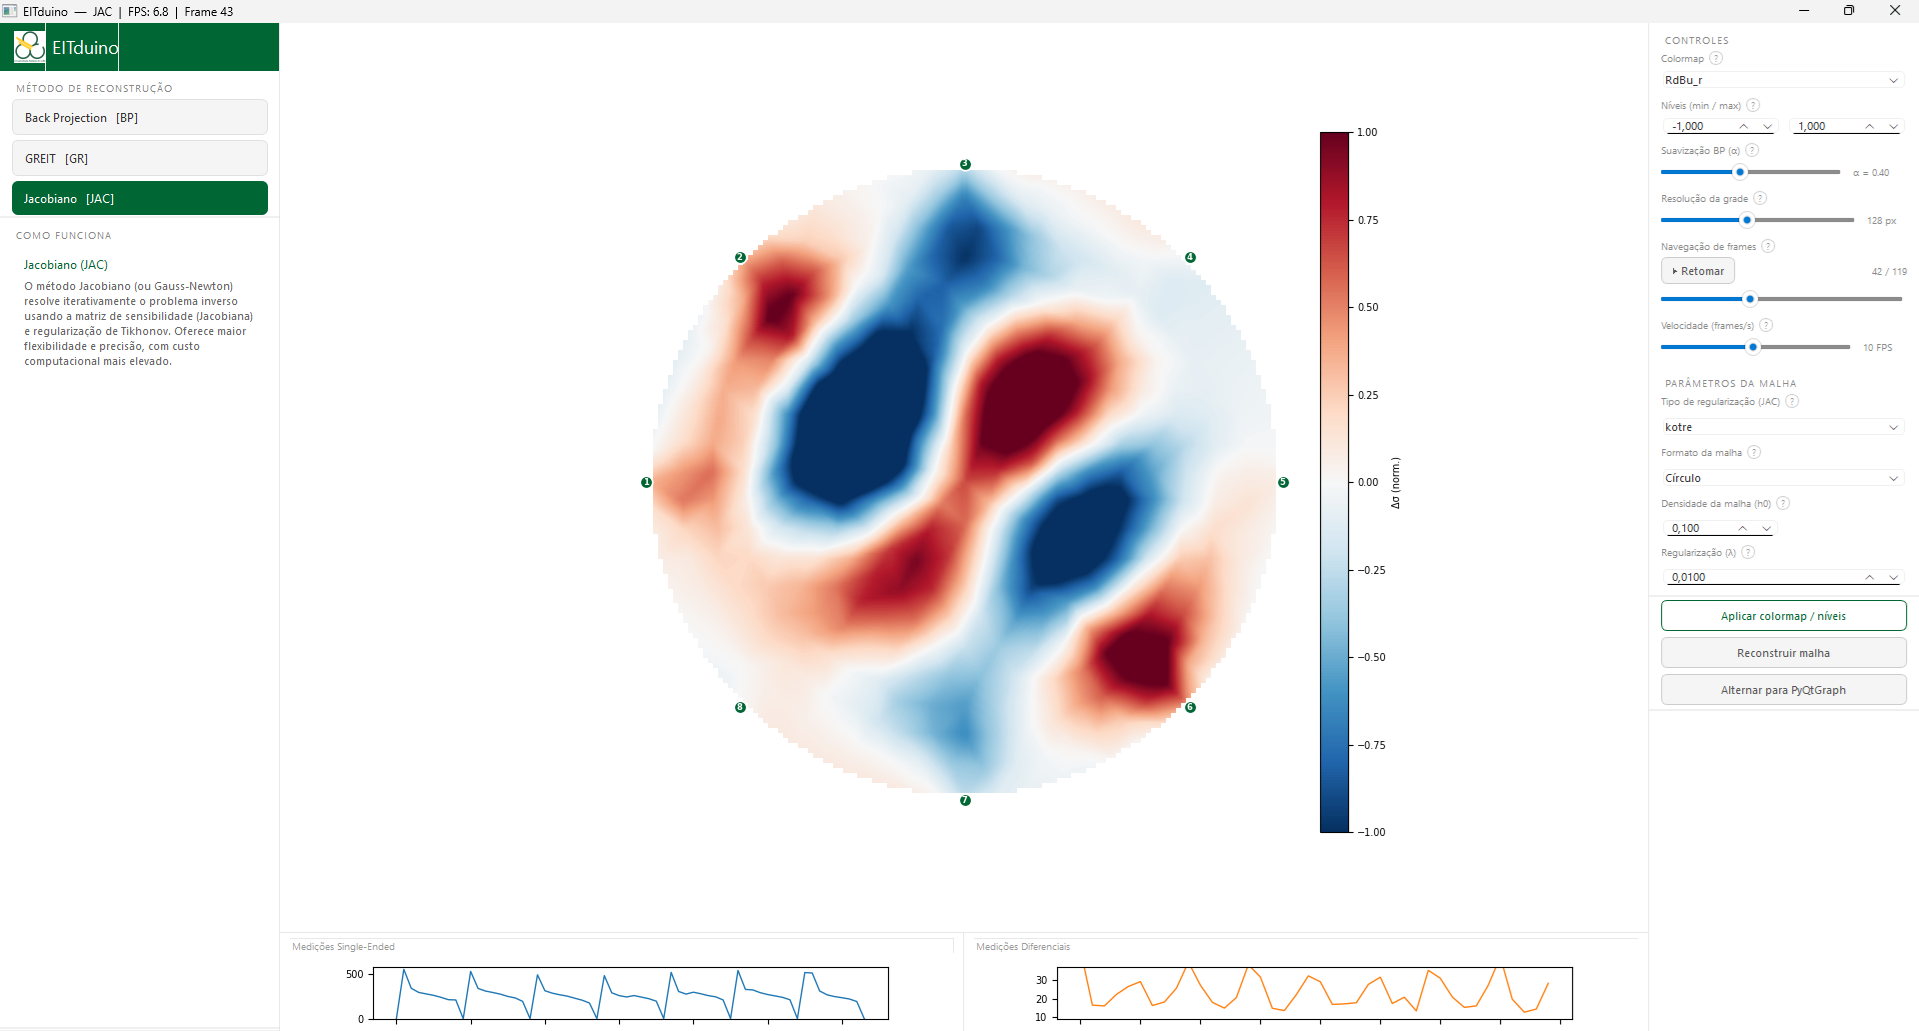
\includegraphics[width=0.94\linewidth]{pictures/JAC_Interface_Frame43.png}
\begin{tcolorbox}[ufabcnote,title=Figura principal a inserir]
\textbf{Screenshot da interface principal.} Idealmente ocupar quase todo o slide.
\end{tcolorbox}

\vspace{0.2cm}
\begin{tcolorbox}[ufabcbox,title=Legenda breve]
Organização em três regiões: seleção de método à esquerda, imagem ao centro, controles à direita; sinais na faixa inferior.
\end{tcolorbox}

% TODO: confirmar nome do arquivo da screenshot principal.
\end{frame}

\begin{frame}{Comparação entre métodos (mesmo frame)}
\begin{columns}[T,totalwidth=\textwidth]
\column{0.32\textwidth}
% FIGURA: BP_Interface_Frame43 --- inserir em: coluna esquerda
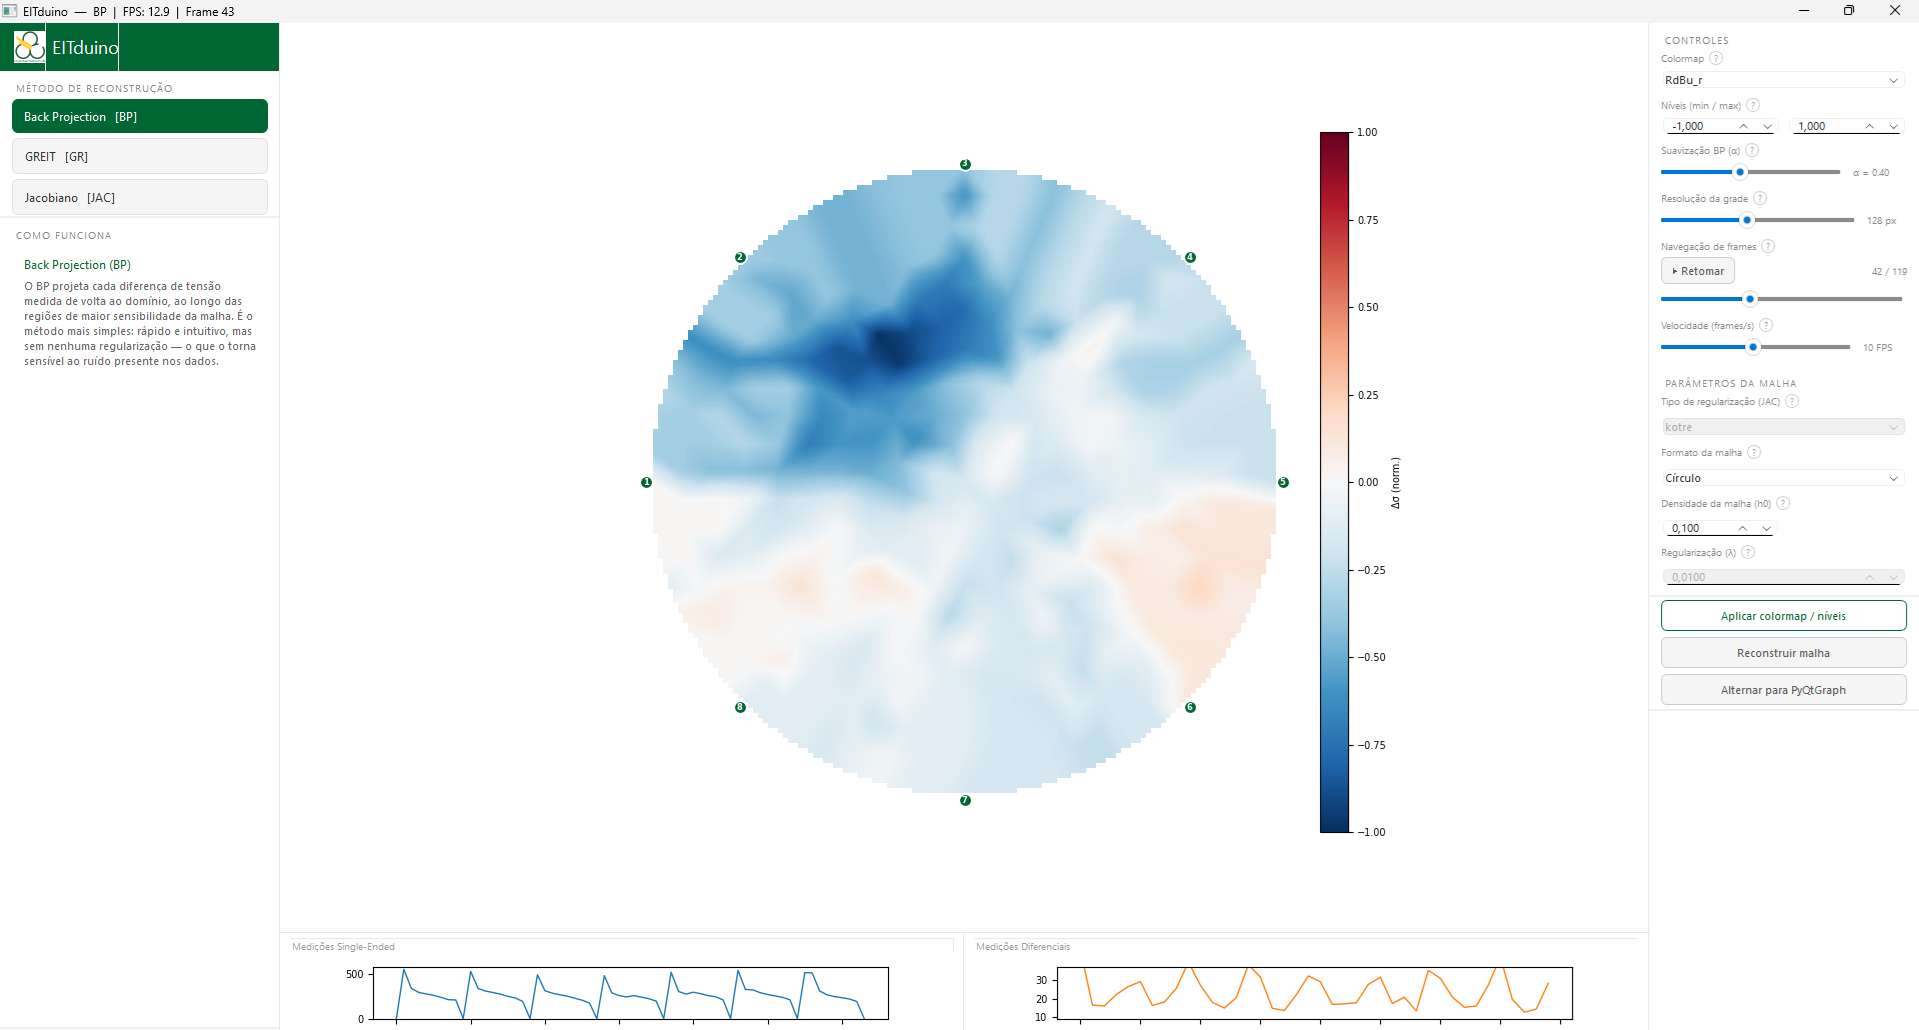
\includegraphics[width=\linewidth]{pictures/BP_Interface_Frame43.png}
\begin{tcolorbox}[ufabcnote,title=BP]
{\scriptsize BP\_Interface\_Frame43}
\end{tcolorbox}

\column{0.32\textwidth}
% FIGURA: JAC_Interface_Frame43 --- inserir em: coluna central
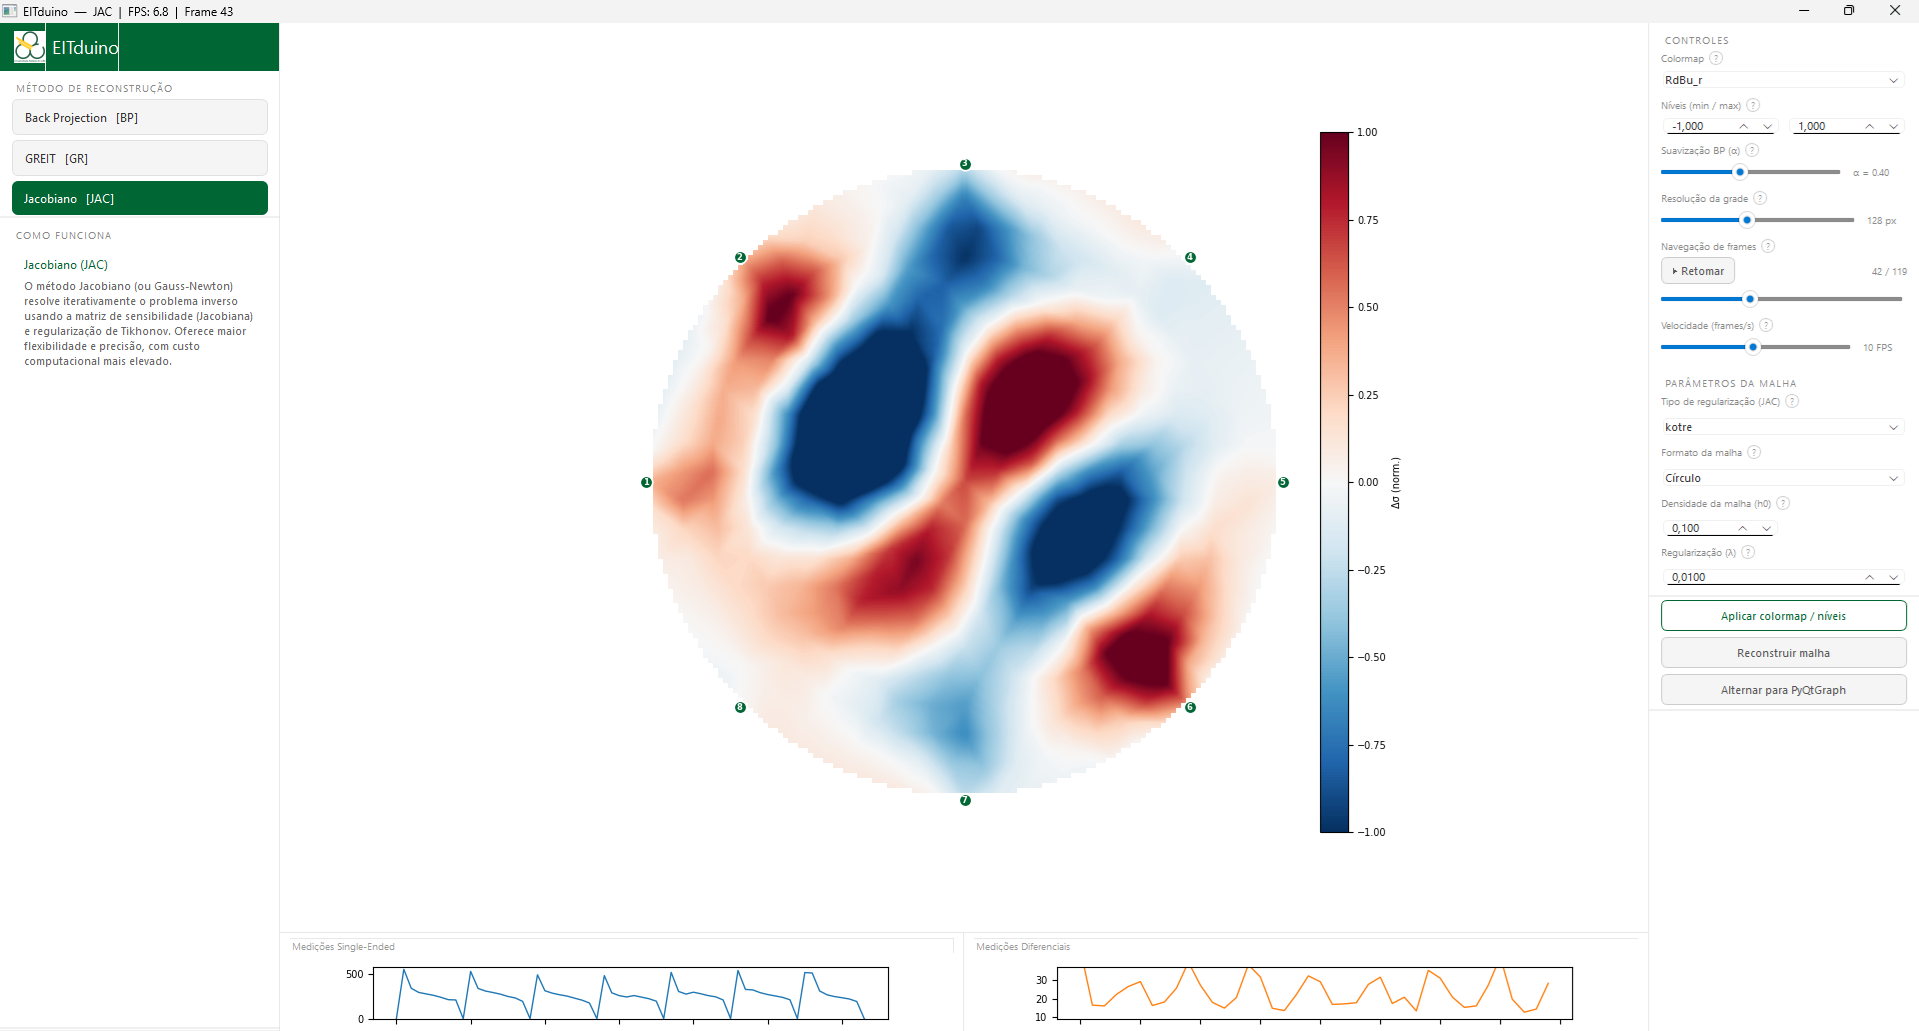
\includegraphics[width=\linewidth]{pictures/JAC_Interface_Frame43.png}
\begin{tcolorbox}[ufabcnote,title=JAC]
{\scriptsize JAC\_Interface\_Frame43}
\end{tcolorbox}

\column{0.32\textwidth}
% FIGURA: GREIT_Interface_Frame43 --- inserir em: coluna direita
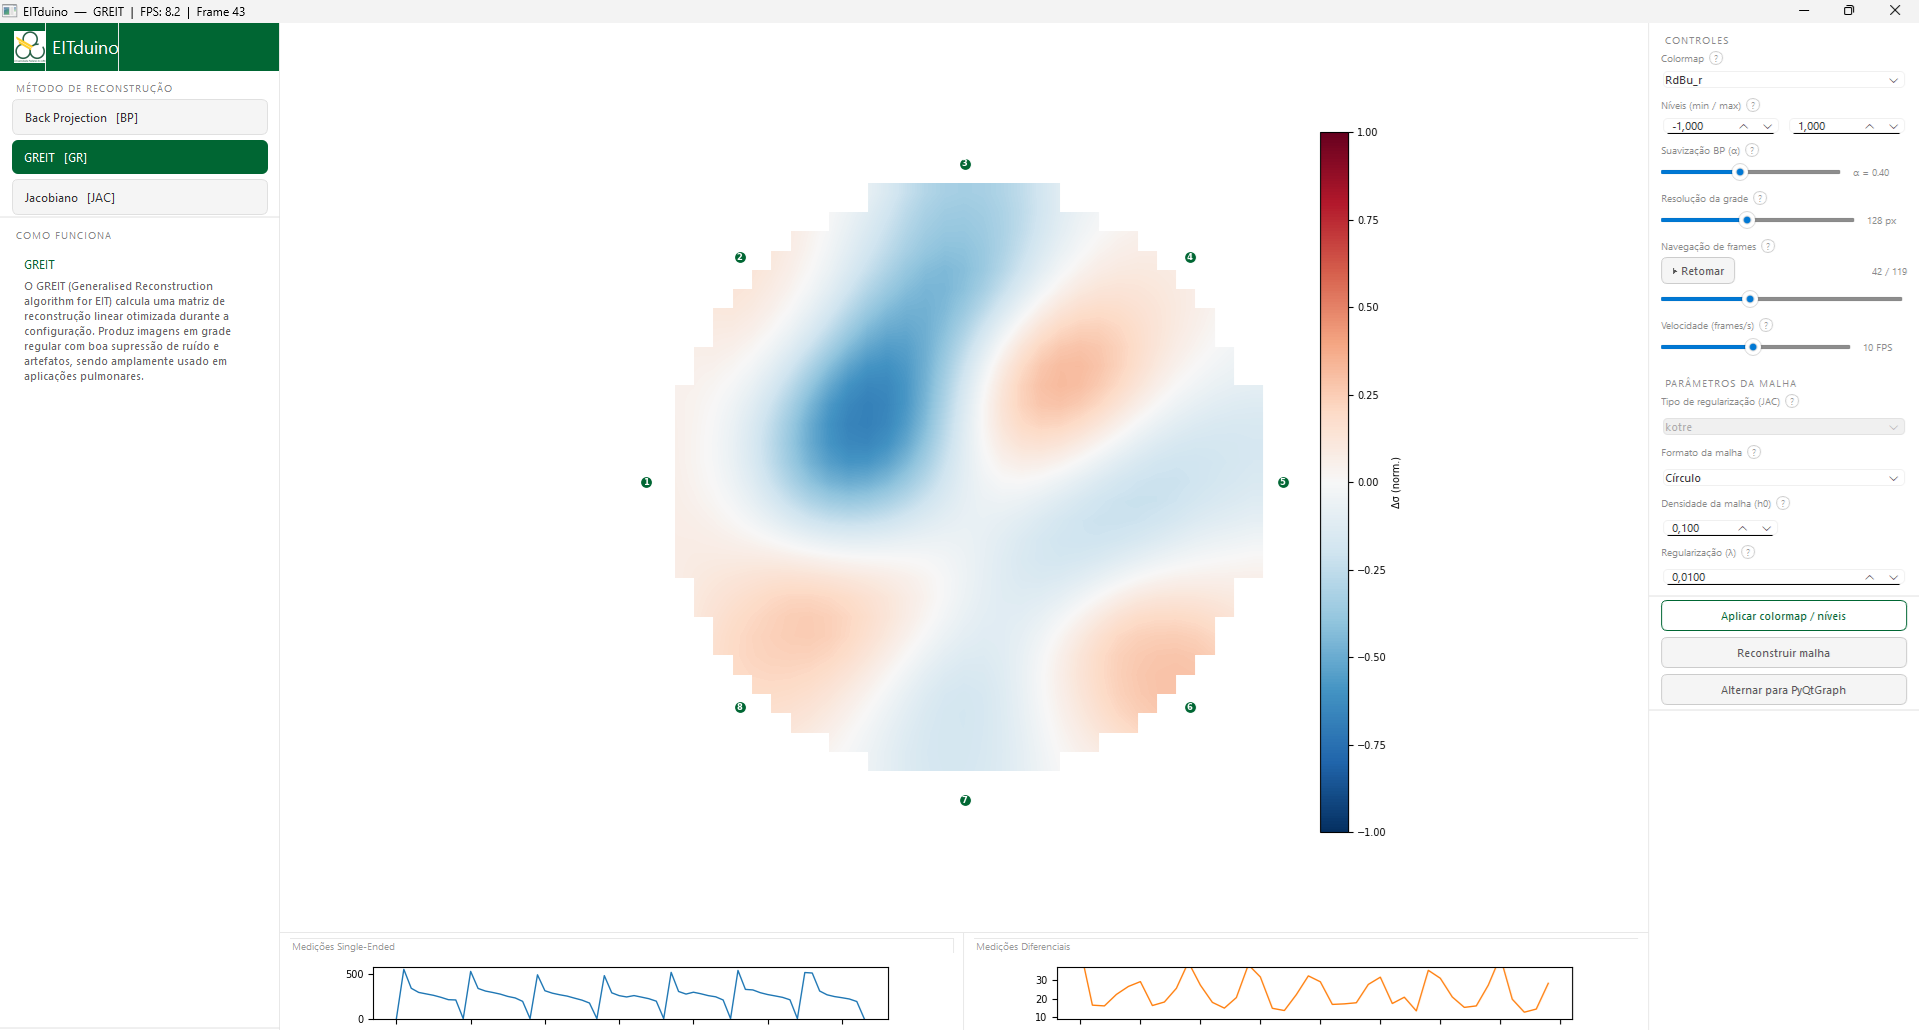
\includegraphics[width=\linewidth]{pictures/GREIT_Interface_Frame43.png}
\begin{tcolorbox}[ufabcnote,title=GREIT]
{\scriptsize GREIT\_Interface\_Frame43}
\end{tcolorbox}
\end{columns}

% TODO: confirmar nomes exatos dos arquivos.
\end{frame}

\begin{frame}{Efeito da densidade de malha (\texttt{h0}) --- JAC}
\begin{columns}[T,totalwidth=\textwidth]
\column{0.48\textwidth}
% FIGURA: JAC_Interface_Frame44_H0_05 --- inserir em: coluna esquerda
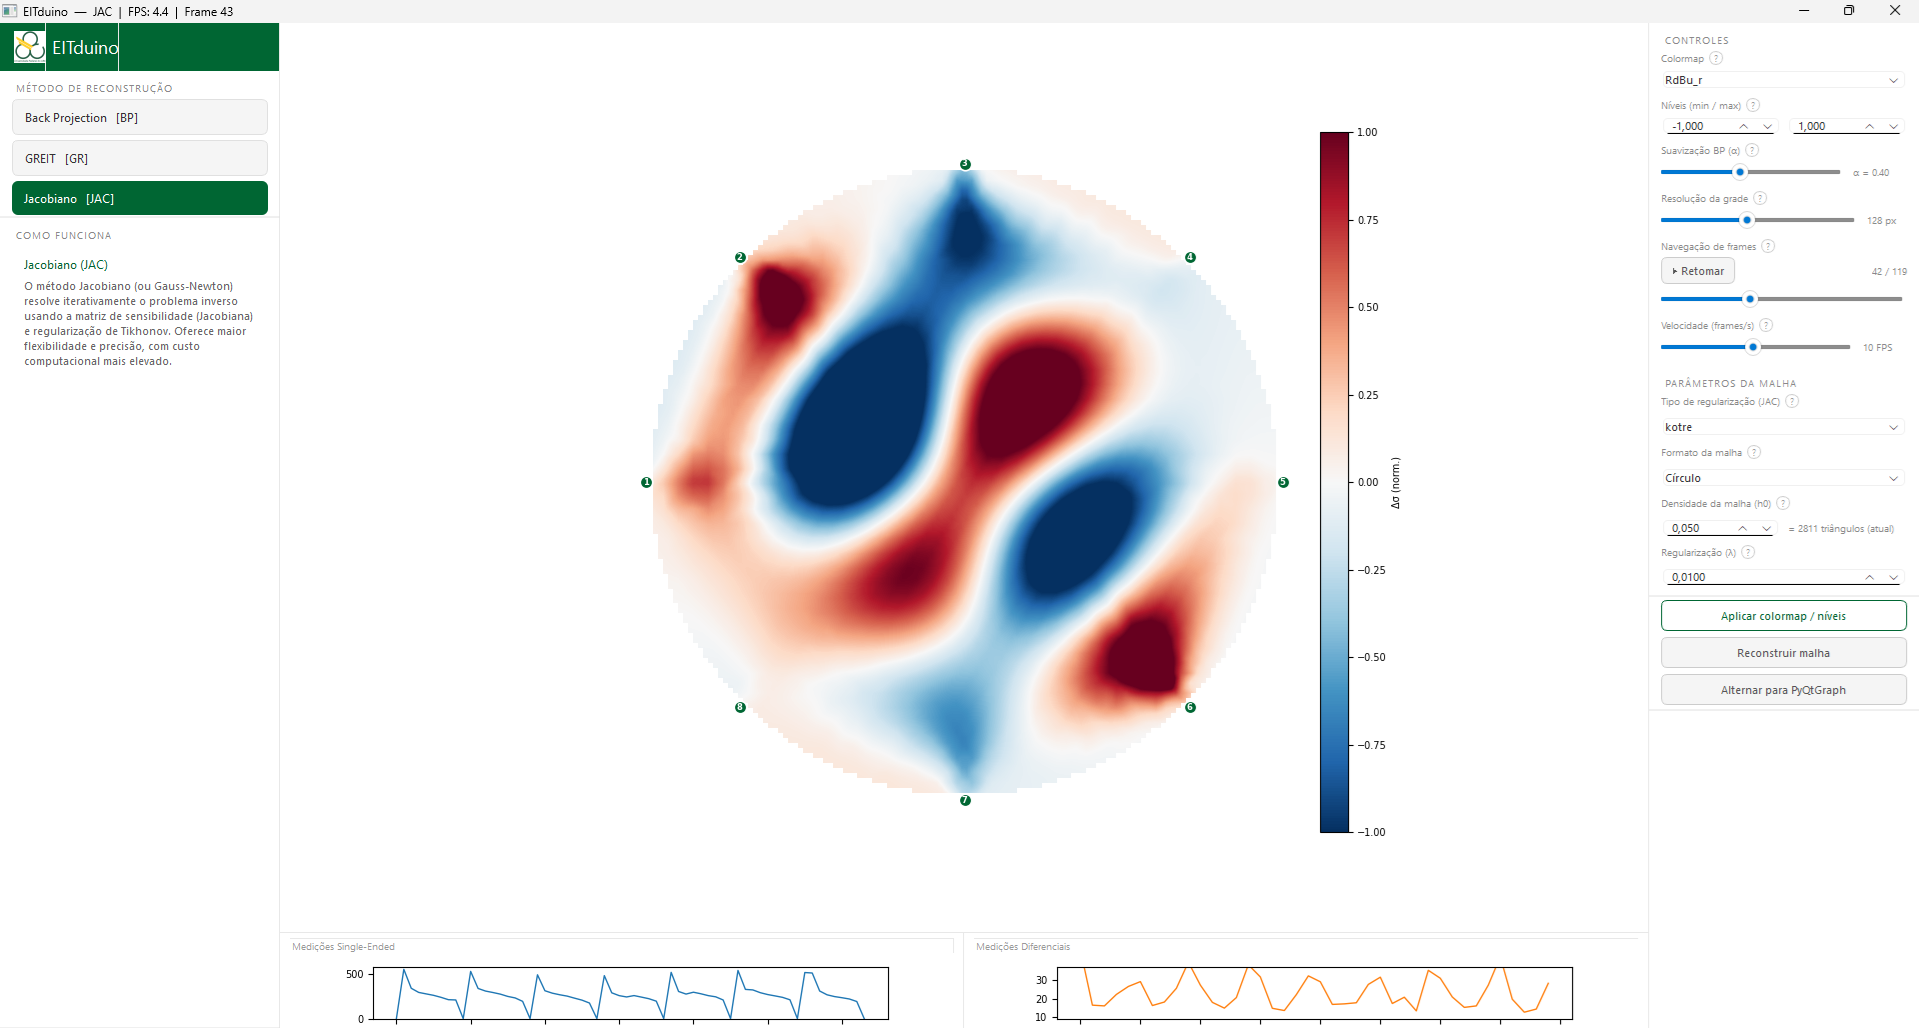
\includegraphics[width=\linewidth]{pictures/JAC_Interface_Frame44_H0_05.png}
\begin{tcolorbox}[ufabcnote,title={$h_0=0{,}05$}]
Malha fina, \textasciitilde 2811 triângulos.
\end{tcolorbox}

\column{0.48\textwidth}
% FIGURA: JAC_Interface_Frame44_H0_2 --- inserir em: coluna direita
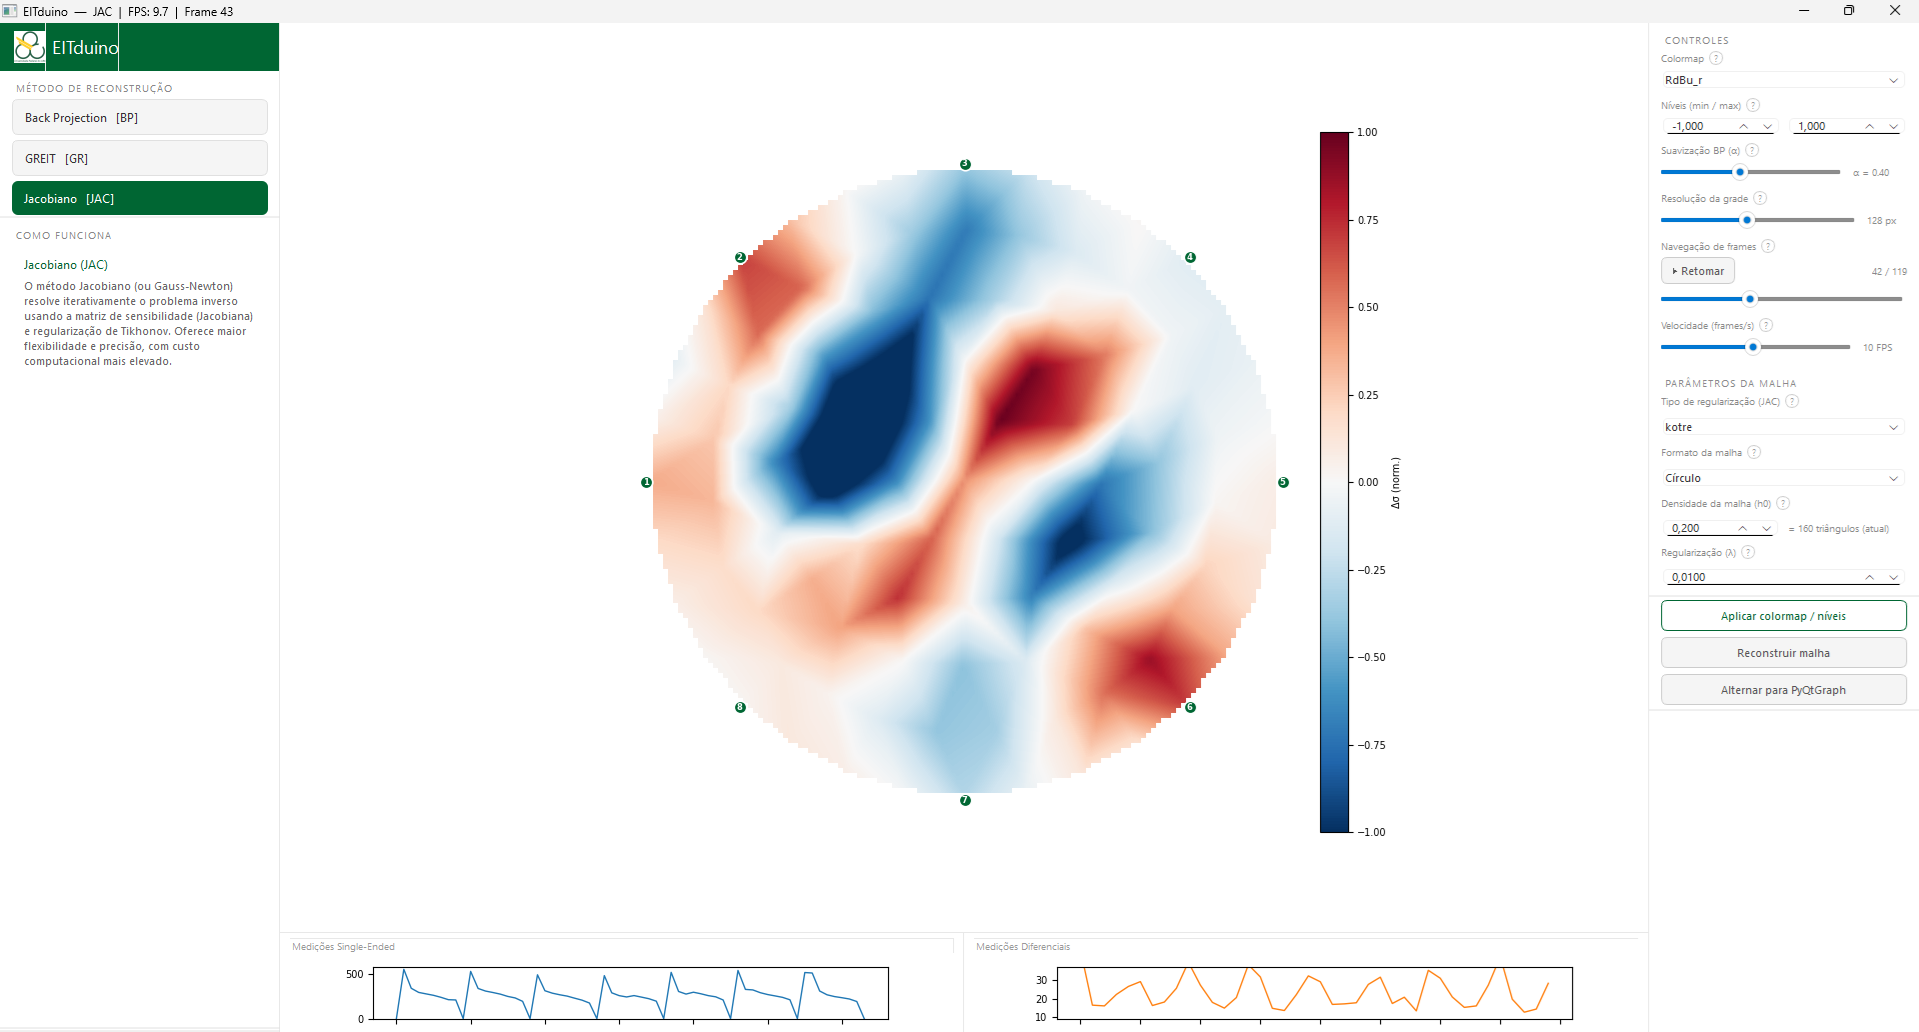
\includegraphics[width=\linewidth]{pictures/JAC_Interface_Frame44_H0_2.png}
\begin{tcolorbox}[ufabcnote,title={$h_0=0{,}20$}]
Malha grossa, \textasciitilde 160 triângulos.
\end{tcolorbox}
\end{columns}

% TODO: verificar nomes finais das figuras (na tese aparecem frame 44 para esse comparativo).
\end{frame}

\begin{frame}{Efeito da suavização temporal ($\alpha$) --- BP}
\begin{columns}[T,totalwidth=\textwidth]
\column{0.48\textwidth}
% FIGURA: BP_Interface_Frame43_alpha0_1 --- inserir em: coluna esquerda
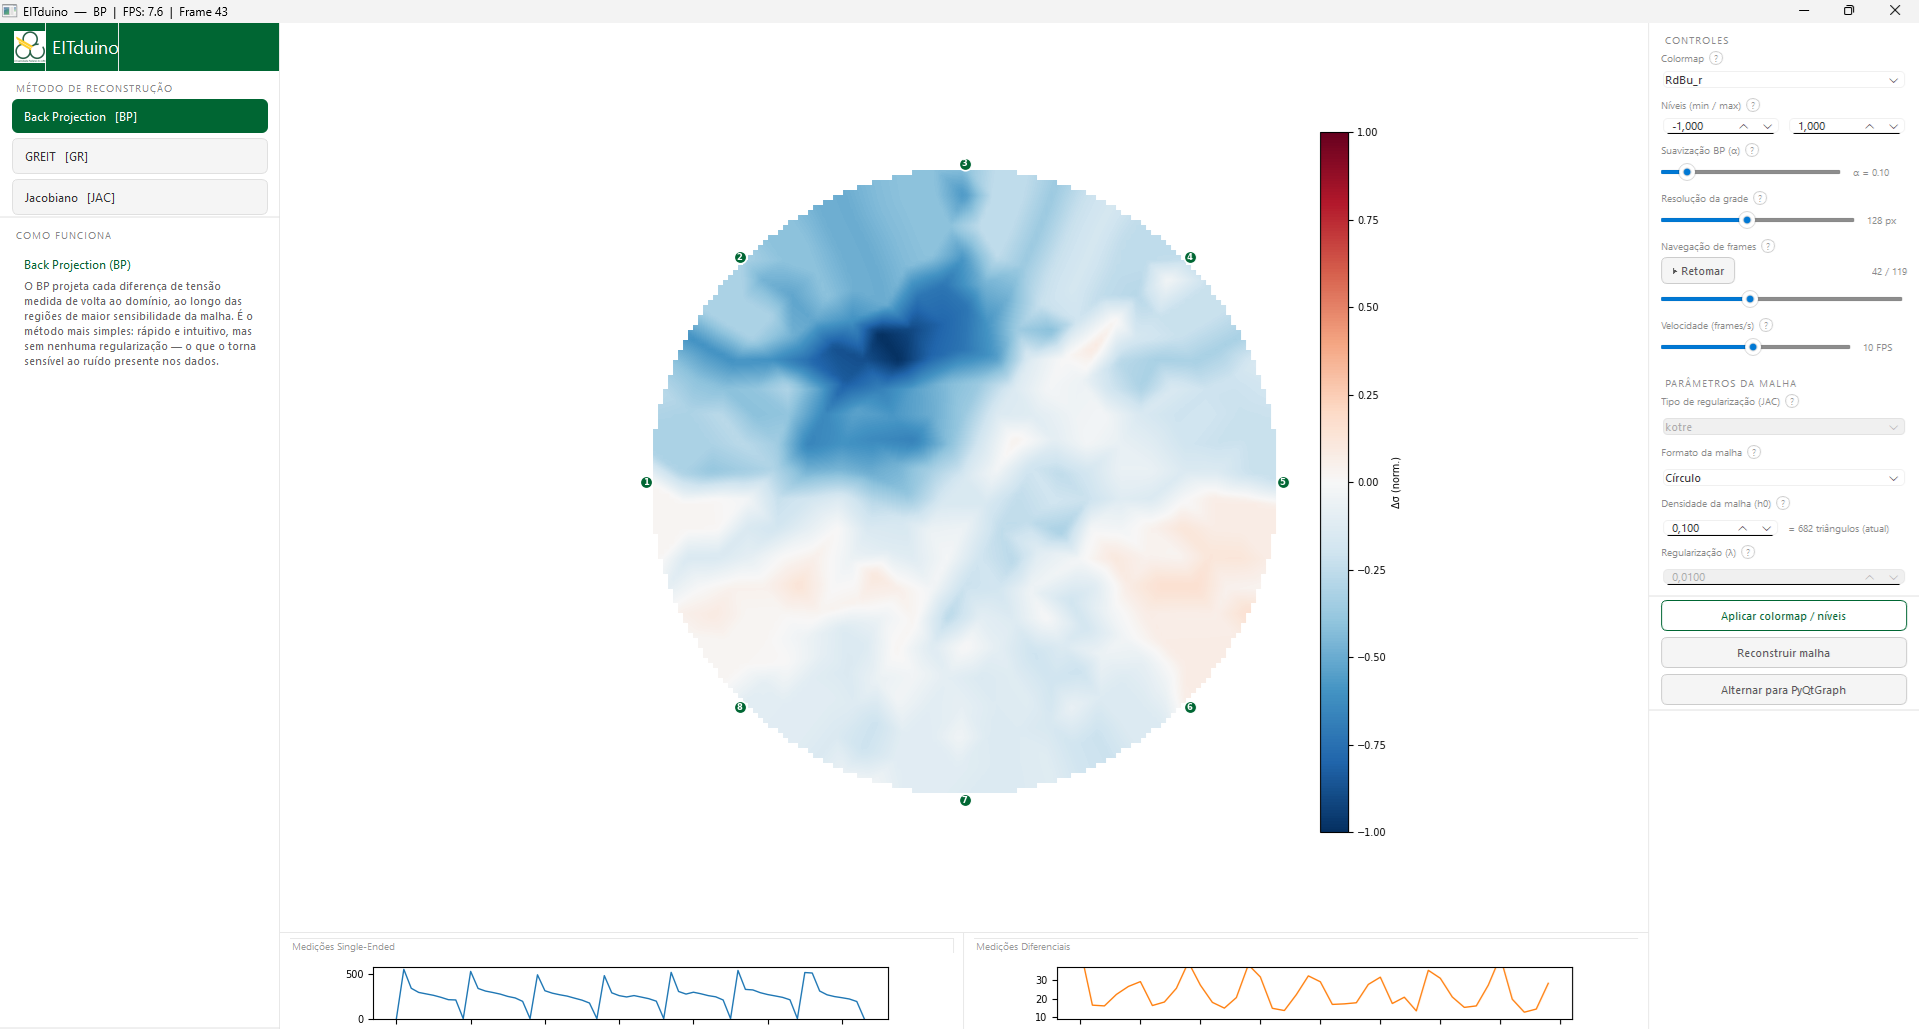
\includegraphics[width=\linewidth]{pictures/BP_Interface_Frame43_alpha0_1.png}
\begin{tcolorbox}[ufabcnote,title={$\alpha=0{,}10$ e $h0=0{,}10$}]
Resposta mais imediata ao frame corrente.
\end{tcolorbox}

\column{0.48\textwidth}
% FIGURA: BP_Interface_Frame43_alpha0_9 --- inserir em: coluna direita
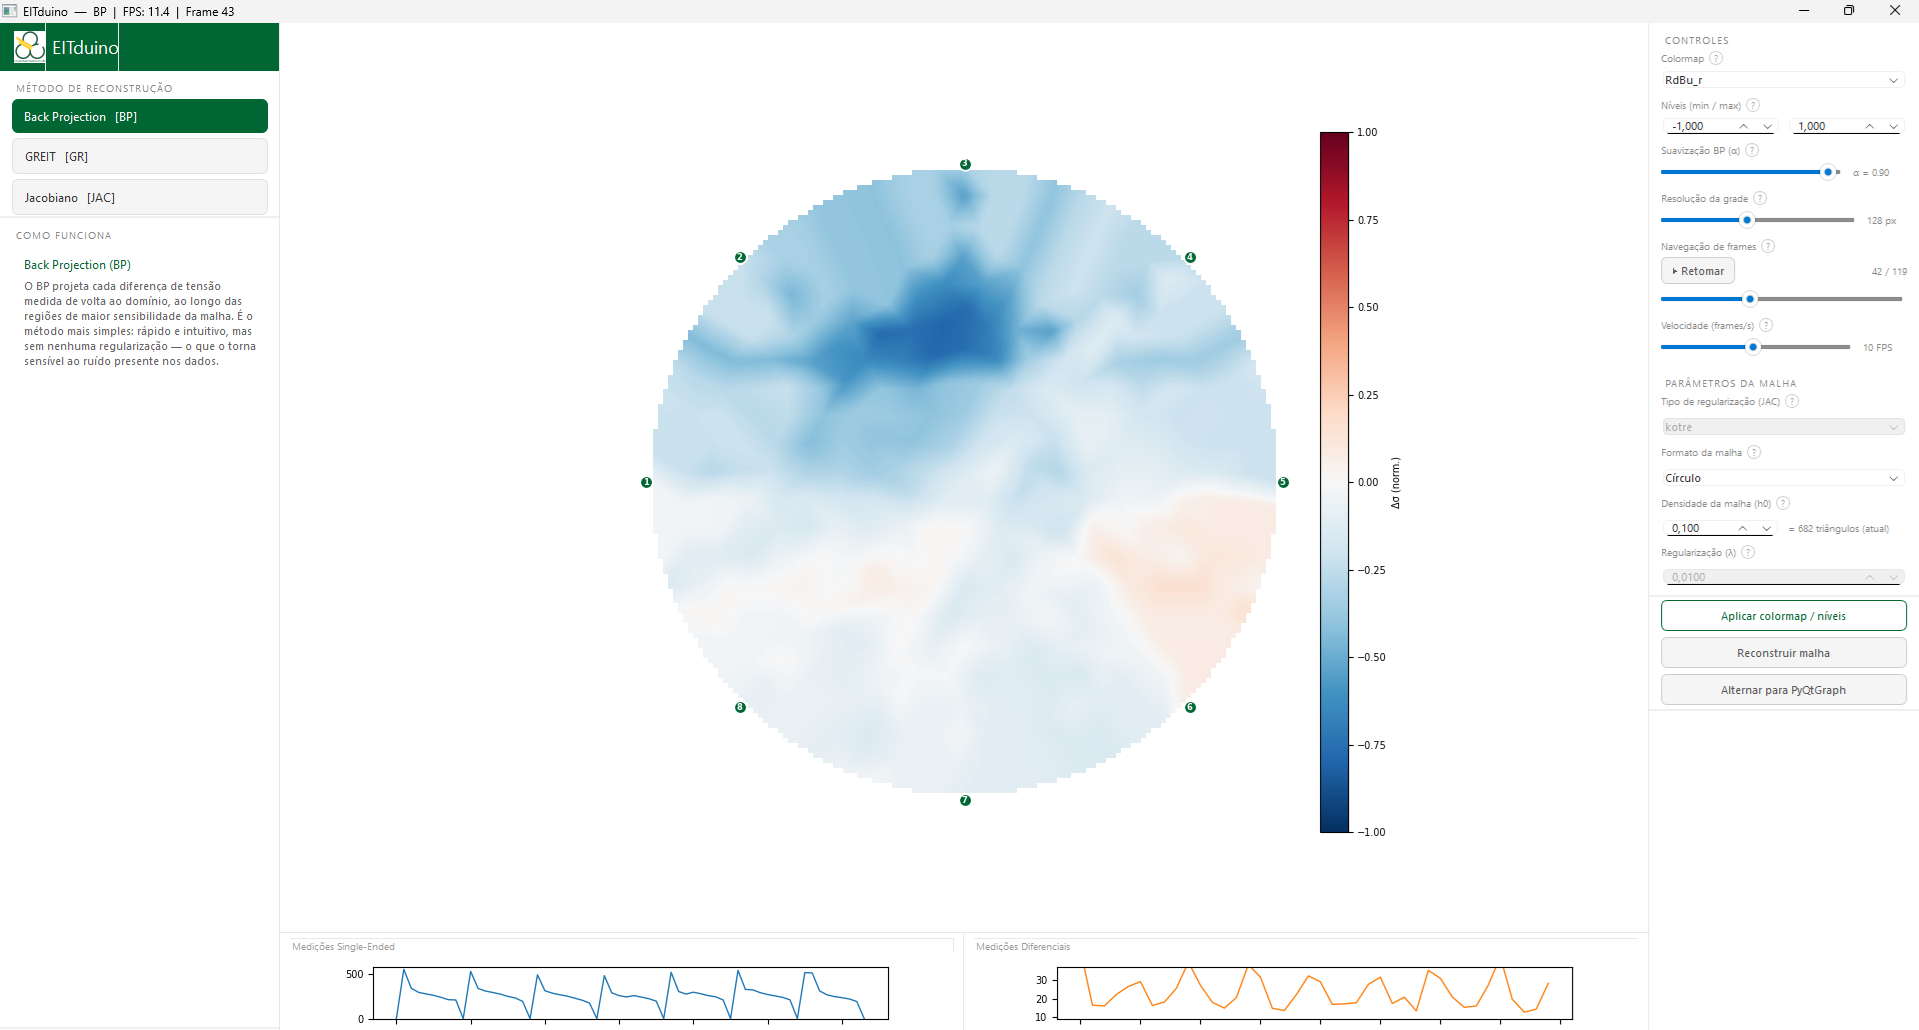
\includegraphics[width=\linewidth]{pictures/BP_Interface_Frame43_alpha0_9.png}
\begin{tcolorbox}[ufabcnote,title={$\alpha=0{,}90$ e $h0=0{,}10$}]
Transição mais suave entre frames.
\end{tcolorbox}
\end{columns}

\end{frame}

\begin{frame}{Efeito da regularização ($\lambda$) --- JAC}
\begin{columns}[T,totalwidth=\textwidth]
\column{0.32\textwidth}
% FIGURA: JAC_pyQT_Reg0_0001 --- inserir em: coluna 1
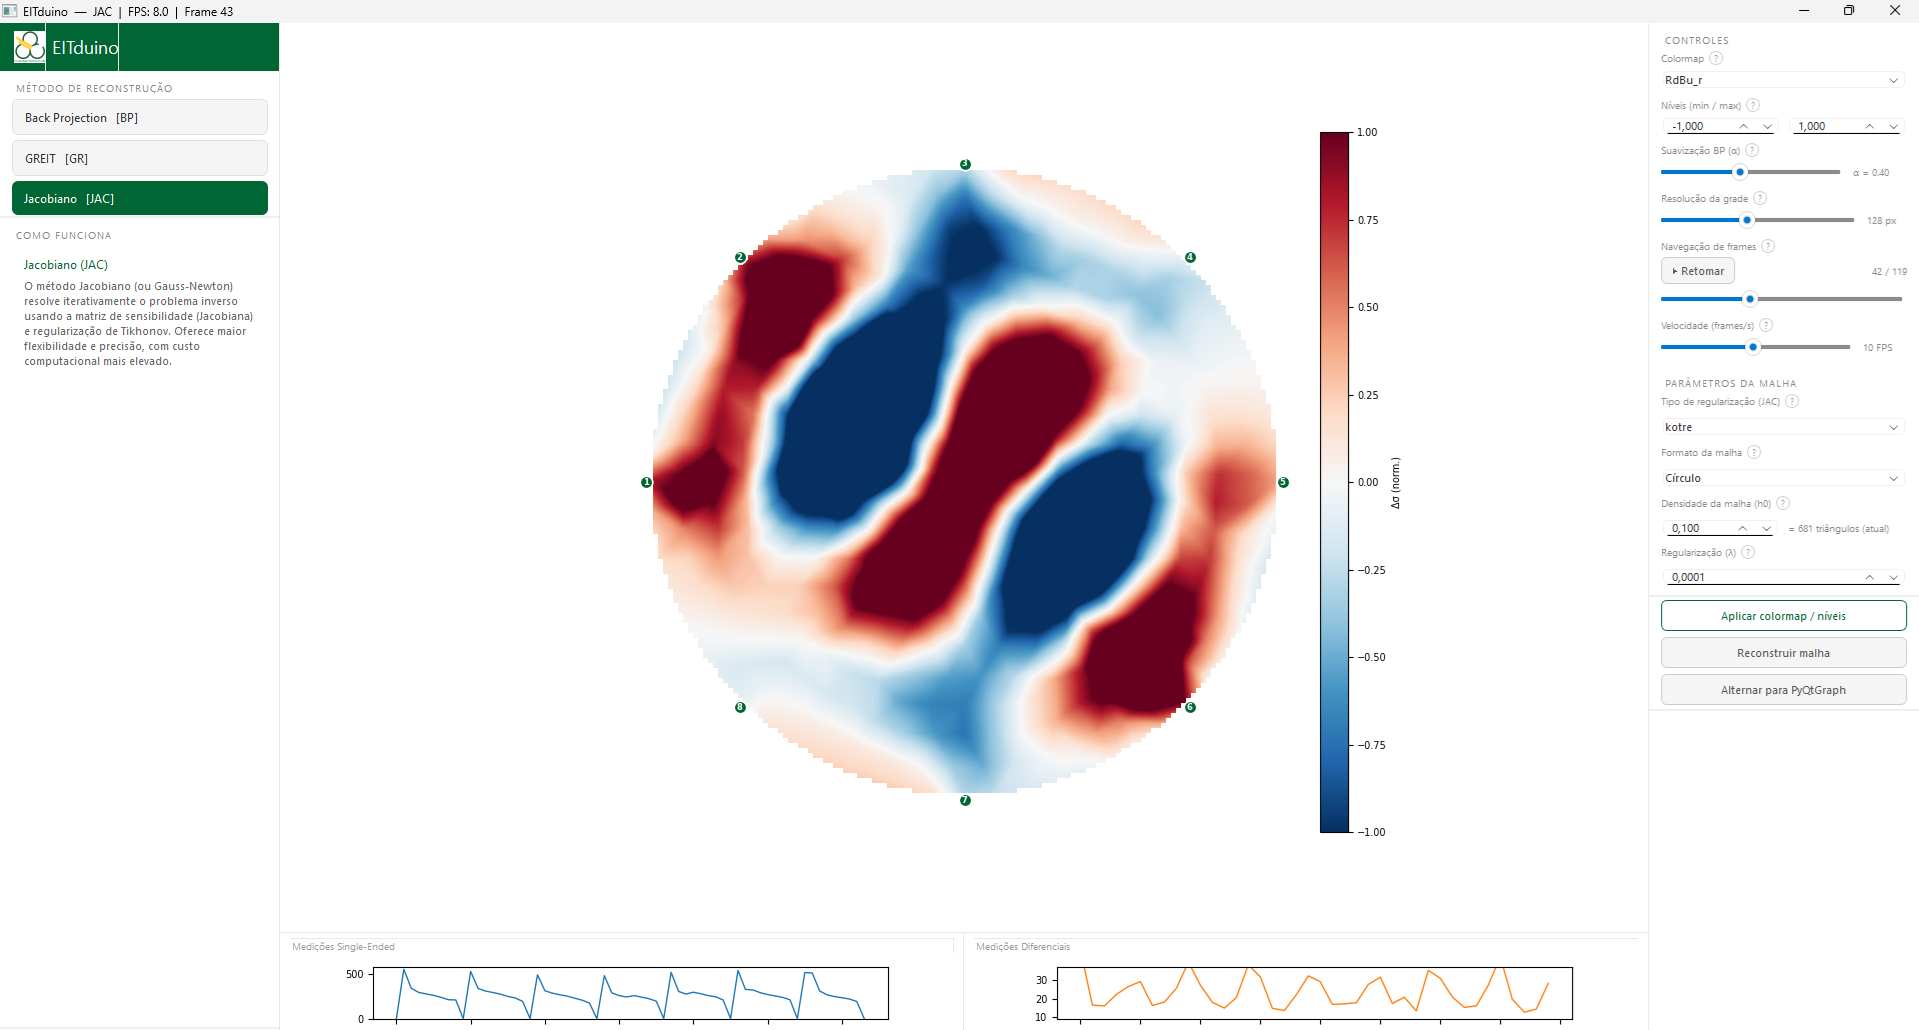
\includegraphics[width=\linewidth]{pictures/JAC_pyQT_Reg0_0001.png}
\begin{tcolorbox}[ufabcnote,title={$\lambda=0{,}0001$}]
Maior sensibilidade; imagem mais ruidosa.
\end{tcolorbox}

\column{0.32\textwidth}
% FIGURA: JAC_pyQT_Reg0_01 --- inserir em: coluna 2
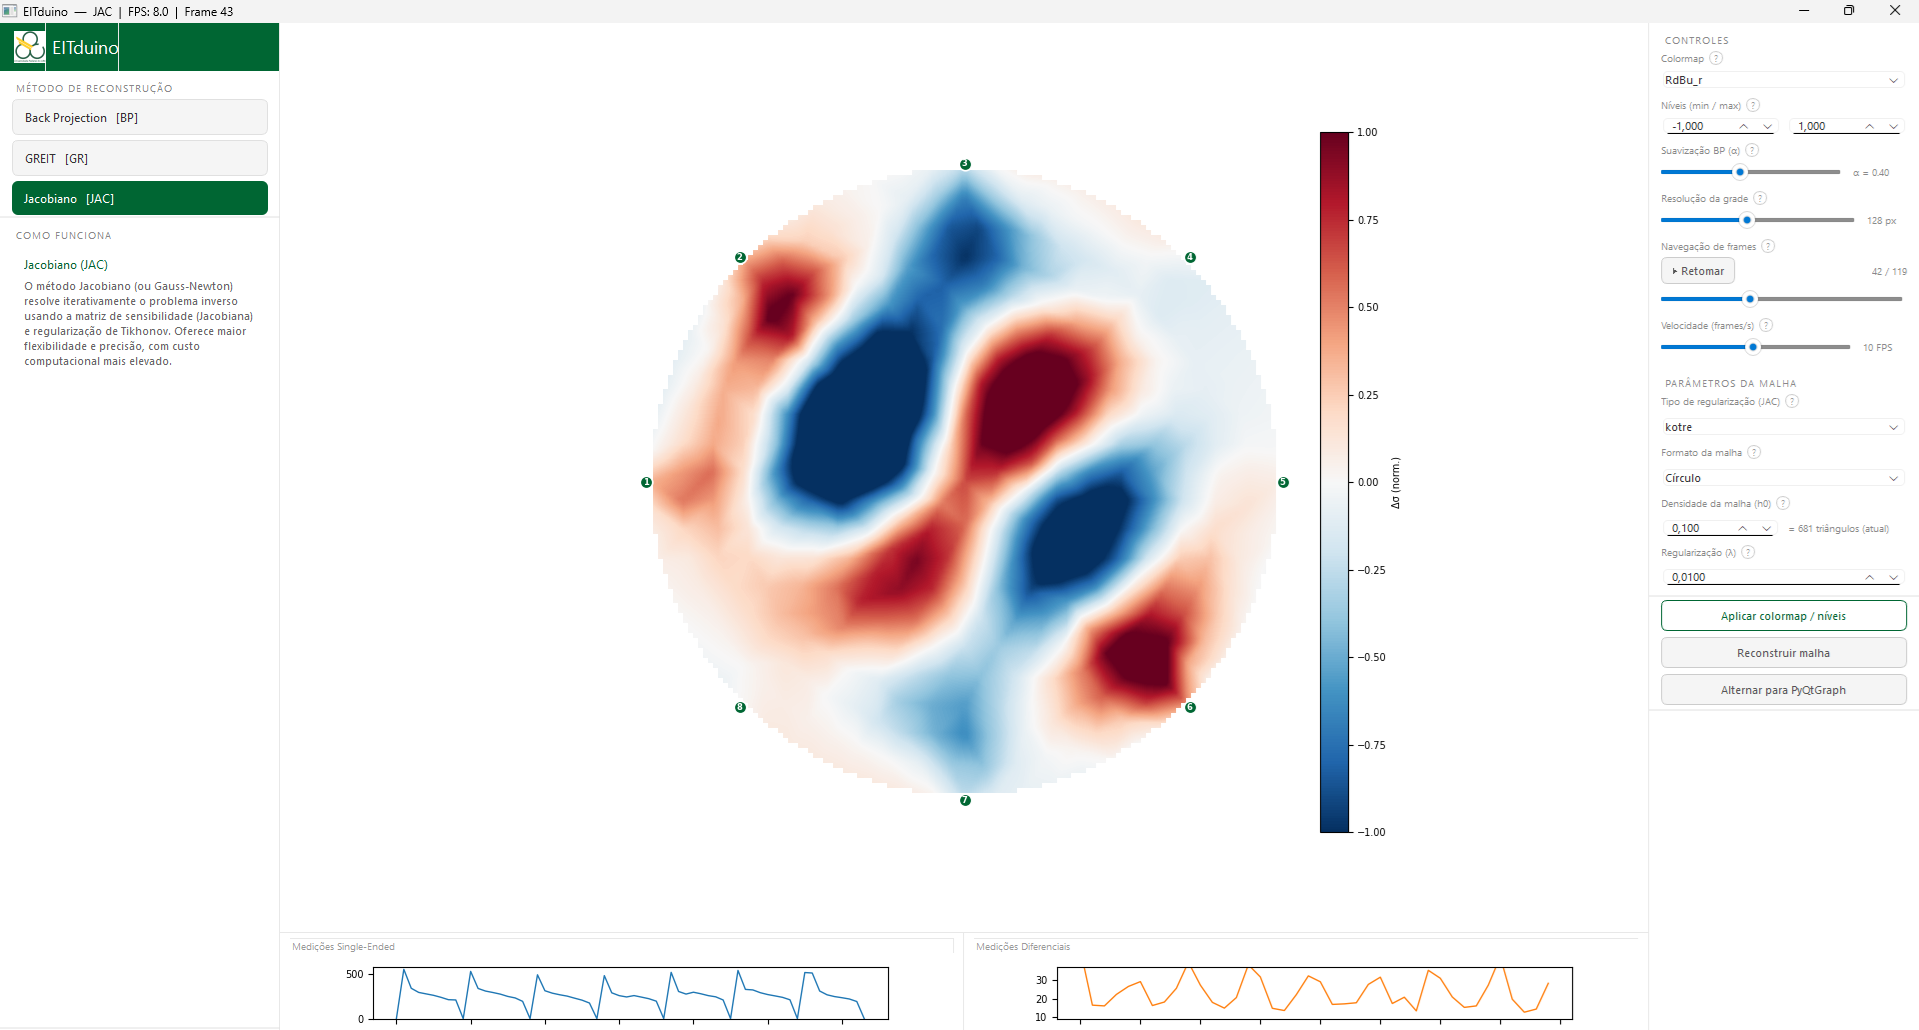
\includegraphics[width=\linewidth]{pictures/JAC_pyQT_Reg0_01.png}
\begin{tcolorbox}[ufabcnote,title={$\lambda=0{,}01$}]
Compromisso intermediário.
\end{tcolorbox}

\column{0.32\textwidth}
% FIGURA: JAC_pyQT_Reg1 --- inserir em: coluna 3
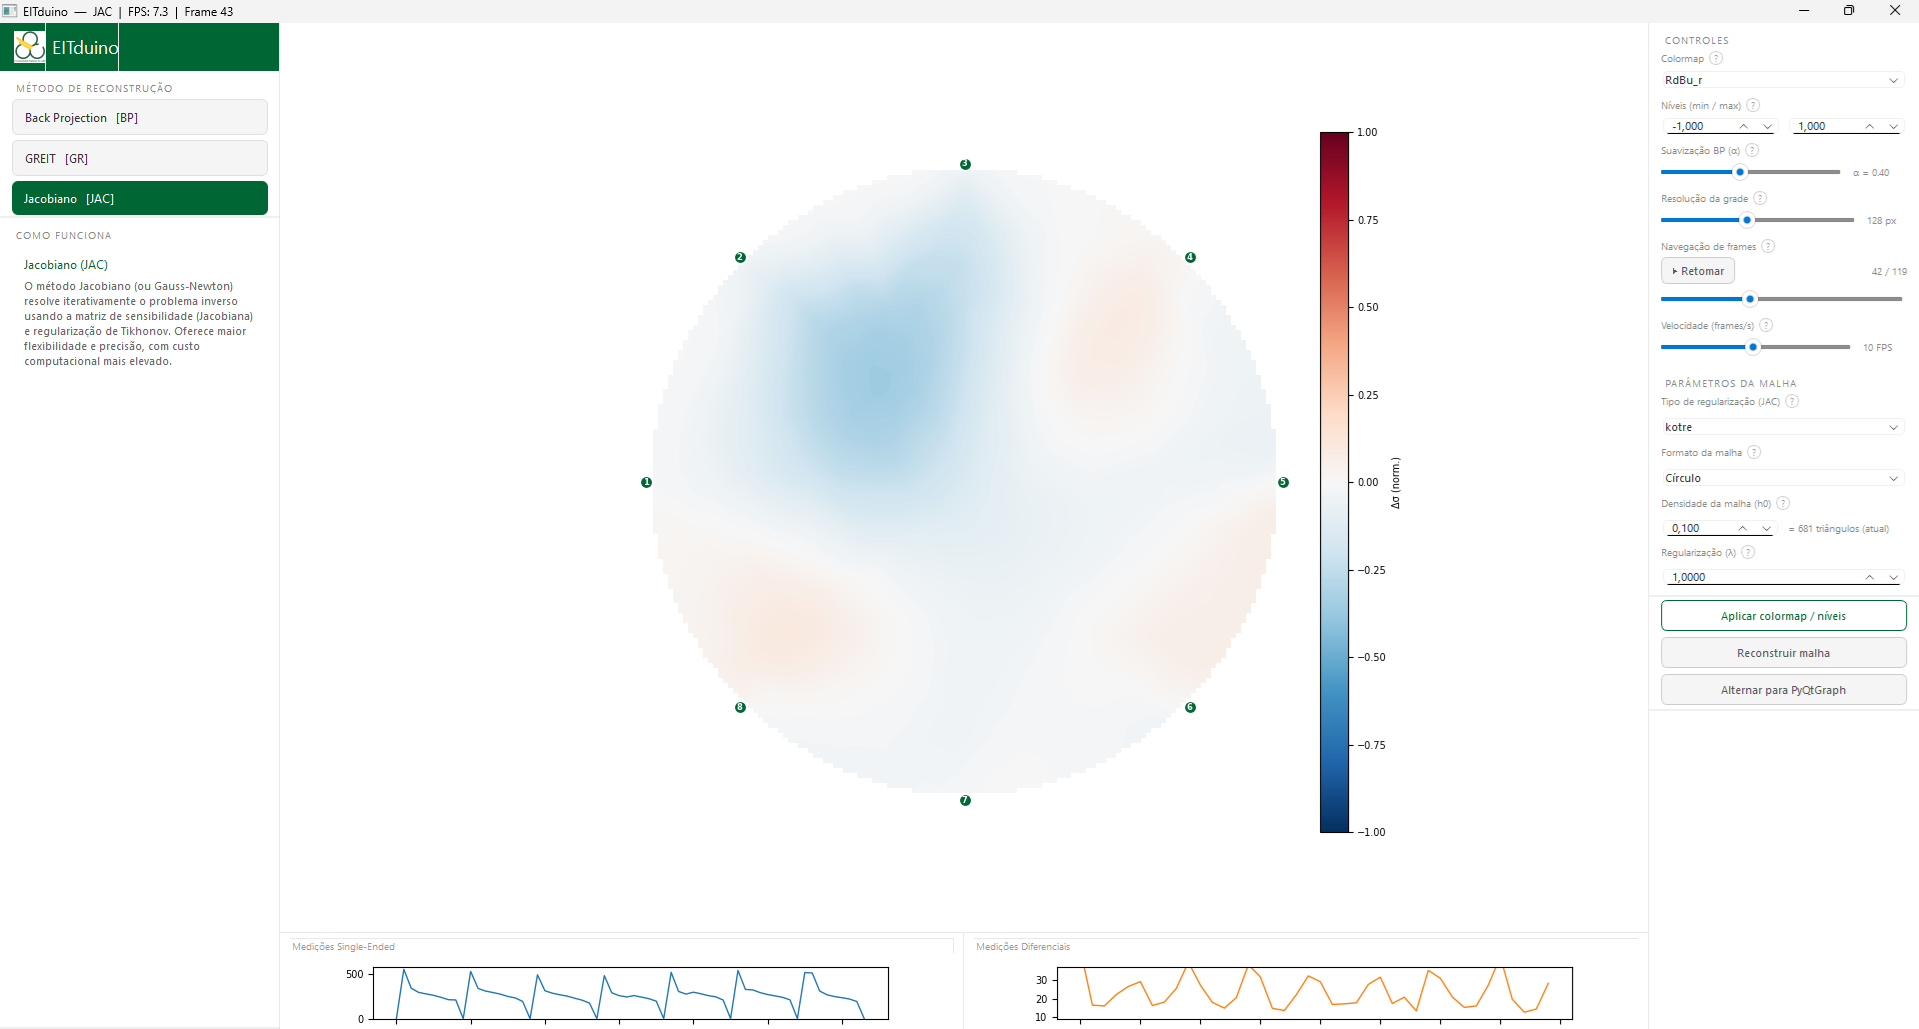
\includegraphics[width=\linewidth]{pictures/JAC_pyQT_Reg1.png}
\begin{tcolorbox}[ufabcnote,title={$\lambda=1$}]
Super-suavização e perda de contraste.
\end{tcolorbox}
\end{columns}

% TODO: se preferir GREIT neste slide, substituir os placeholders por GREIT_pyQT_Reg*.
\end{frame}

\begin{frame}{Interface alternativa em PyQtGraph}
% FIGURA: BP_PyQtGraph_SolverTab --- inserir em: largura total do slide
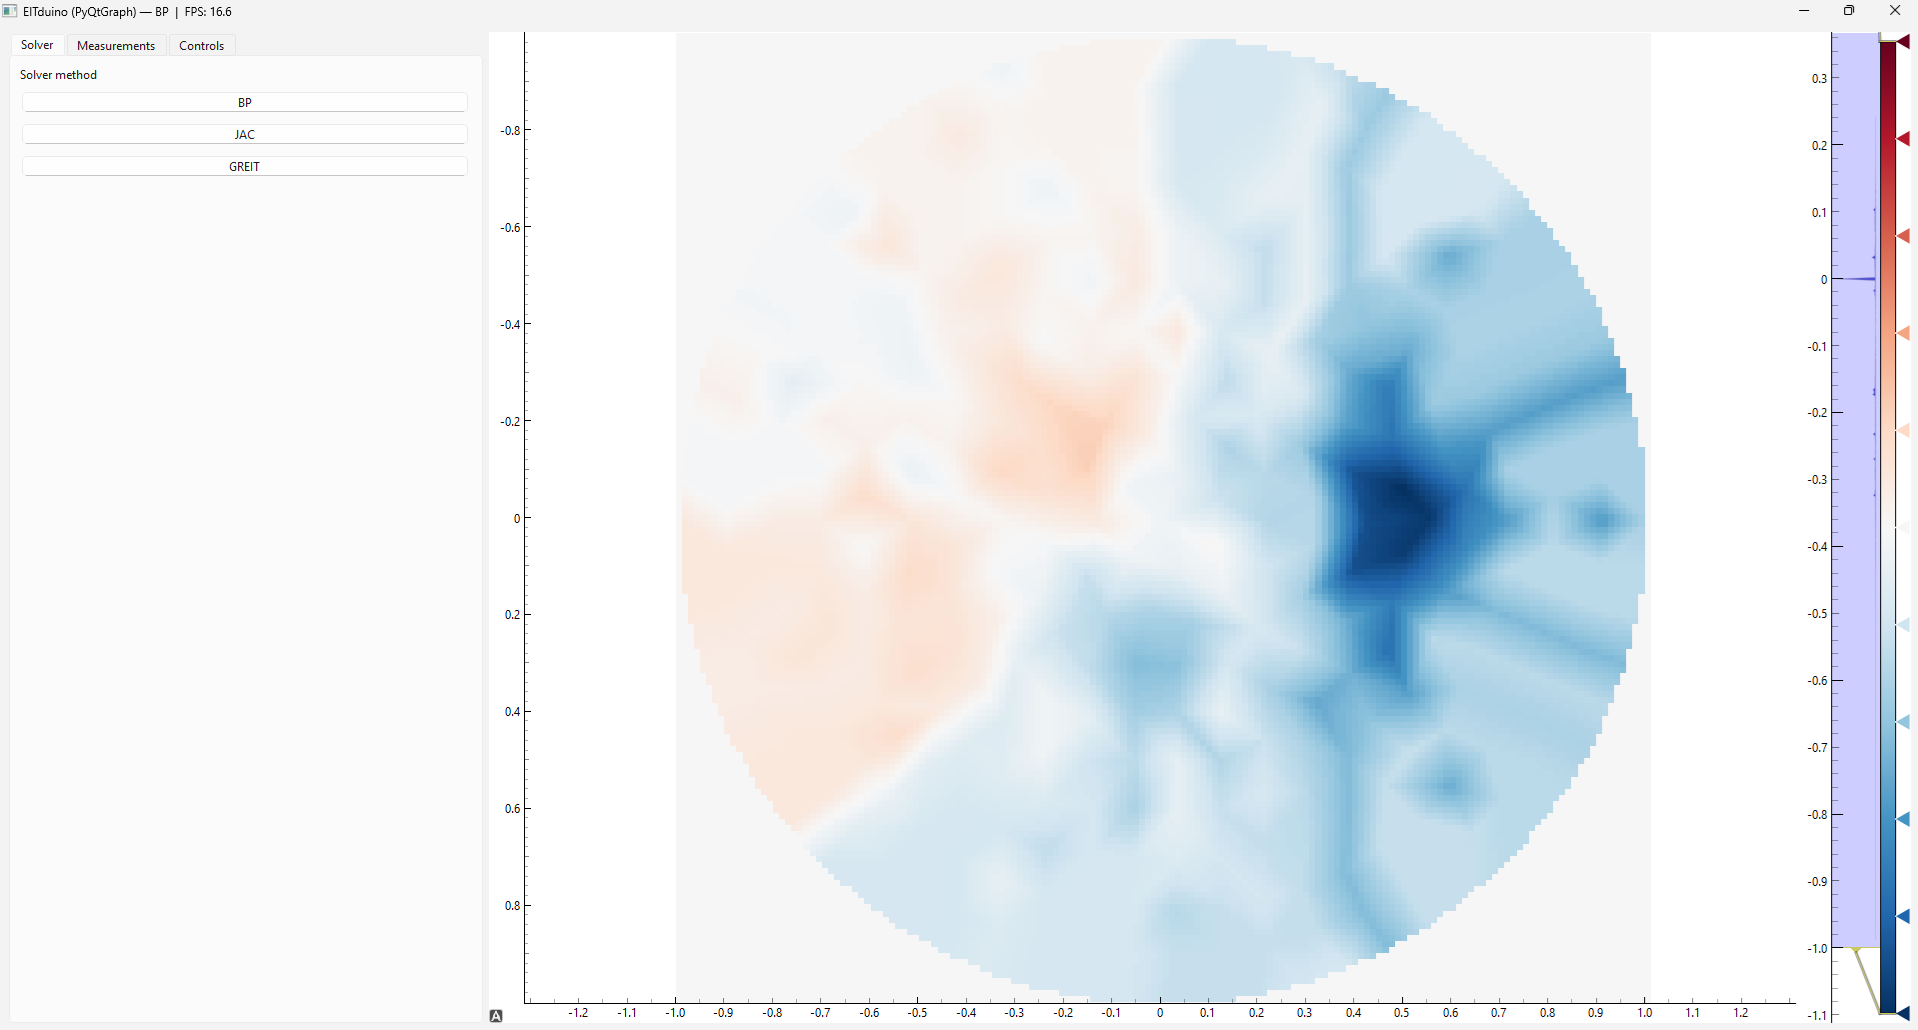
\includegraphics[width=0.82\linewidth]{pictures/BP_PyQtGraph_SolverTab.png}

\vspace{0.2cm}
\begin{tcolorbox}[ufabcbox,title=Leitura arquitetural]
Prova de conceito de um segundo backend reutilizando a mesma camada \texttt{EITsolver} --- validação prática do desacoplamento arquitetural.
\end{tcolorbox}

% TODO: escolher screenshots finais das abas.
\end{frame}

% BLOCO 6 --- Demonstração ao vivo --- alvo: 6 min (~1 slide)
\section{Demo e conclusão}

\begin{frame}{Demonstração}
\centering
\vspace{0.4cm}
{\Huge\bfseries Demonstração}
\vspace{0.5cm}

\begin{tcolorbox}[ufabcbox,title=Roteiro]
\begin{itemize}
  \item Abrir o EITduino.
  \item Alternar BP $\rightarrow$ JAC $\rightarrow$ GREIT mantendo o mesmo frame.
  \item Variar \texttt{h0} e reconstruir malha.
  \item Variar $\lambda$.
  \item Navegar frames e mostrar animação.
  \item Alternar para a interface PyQtGraph.
\end{itemize}
\end{tcolorbox}

% Nota em comentário: Vídeo de backup obrigatório caso a demo ao vivo falhe.
\end{frame}

% BLOCO 7 --- Limitações e trabalhos futuros --- alvo: 3 min (~2 slides)
\begin{frame}{Limitações e trabalhos futuros}
\vspace{-0.4em}
\begin{columns}[T,totalwidth=\textwidth]
\column{0.48\textwidth}
\begin{tcolorbox}[ufabcbox,title=Escopo atual do trabalho]
\scriptsize
\begin{itemize}\setlength{\itemsep}{1pt}\setlength{\parskip}{0pt}\setlength{\topsep}{1pt}
  \item Análise baseada em um único conjunto de dados experimentais (119 frames, phantom simplificado).
  \item Sem integração com hardware de aquisição em tempo real.
  \item Comparação entre métodos qualitativa --- sem métricas quantitativas formais de contraste, erro de posição ou estabilidade.
  \item Interface PyQtGraph como prova de conceito, menos completa que a principal.
  \item Sem testes unitários automatizados para os pipelines de malha e reconstrução.
\end{itemize}
\end{tcolorbox}

\column{0.48\textwidth}
\begin{tcolorbox}[ufabcnote,title=Continuidade natural]
\scriptsize
\begin{itemize}\setlength{\itemsep}{1pt}\setlength{\parskip}{0pt}\setlength{\topsep}{1pt}
  \item Integração com sistemas reais de aquisição em tempo real.
  \item Métricas quantitativas de avaliação (contraste, definição, estabilidade, custo computacional).
  \item Expansão da interface PyQtGraph para paridade com a principal.
  \item Suporte a outros formatos e geometrias de malha.
  \item Inclusão de métodos adicionais de reconstrução.
  \item Testes automatizados e validações formais do pipeline.
\end{itemize}
\end{tcolorbox}
\end{columns}

% FONTE: capítulo 6 da tese
\end{frame}

% BLOCO 8 --- Conclusão --- alvo: 2 min (~2 slides)
\begin{frame}{Conclusão}
\begin{tcolorbox}[ufabcbox,title=Síntese]
\begin{itemize}
  \item O objetivo geral foi atingido: a aplicação permite reconstruir e visualizar dados de TIE de forma interativa.
  \item Contribuição principal: ferramenta modular para exploração interativa de reconstruções em TIE, com foco educacional e de apoio à pesquisa.
  \item Os três métodos implementados localizaram a haste na mesma região do domínio, com diferenças relevantes em contraste, definição espacial e estabilidade temporal.
\end{itemize}
\end{tcolorbox}

\end{frame}

\begin{frame}{Obrigado}
\centering
\vspace{0.5cm}

\includegraphics[width=0.2\textwidth]{logo_ufabc.png}\\[0.7cm]
{\Large\bfseries Obrigado. Perguntas?\\}
\vspace{0.5cm}
{\small Lucas Maio Nunes de Almeida Gonçalves\\}
% TODO: adicionar contato opcional, se desejar.
\end{frame}

% -------------------------------------------------
% BLOCO 9 --- Slides de backup (fora do tempo principal)
% -------------------------------------------------
\appendix

\begin{frame}{Backup --- Detalhes do MVC}
\begin{tcolorbox}[ufabcbox,title=Classes e responsabilidades]
\begin{itemize}
  \item \texttt{main.py}: ponto de entrada; seleção do backend.
  \item \texttt{EITsolver}: criação de malha, \texttt{setVref}, \texttt{updateImage}, \texttt{\_build\_raster\_cache}, solver e pós-processamento.
  \item \texttt{MainWindow} (PyQt6 + Matplotlib): exibição principal e controles.
  \item \texttt{MainWindowPG} (PyQtGraph): backend alternativo com a mesma camada de reconstrução.
  \item Nas classes de interface, \textbf{View} absorve parte das responsabilidades de \textbf{Controller} por convenção do framework.
\end{itemize}
\end{tcolorbox}
\end{frame}

\begin{frame}[fragile]{Backup --- \texttt{setVref} e \texttt{updateImage}}
\begin{tcolorbox}[ufabcnote,title=Trechos de código]
% TODO: inserir trechos reais de \texttt{setVref} e \texttt{updateImage} a partir do código-fonte final.
\end{tcolorbox}
\begin{lstlisting}[language=Python]
# TODO: colar aqui o trecho real de setVref
# TODO: colar aqui o trecho real de updateImage
\end{lstlisting}
\end{frame}

\begin{frame}[fragile]{Backup --- Conversão \textit{single-ended} $\rightarrow$ diferencial}
\begin{tcolorbox}[ufabcbox,title=Ideia do slide]
Explicação curta da conversão utilizada antes da etapa de reconstrução.
\end{tcolorbox}
\begin{lstlisting}[language=Python]
# TODO: inserir o trecho real de conversao single-ended -&amp;gt; diferencial
\end{lstlisting}
\end{frame}

\begin{frame}{Backup --- pyEIT vs EIDORS}
\begin{tcolorbox}[ufabcbox,title=Justificativa da escolha do pyEIT]
\centering
\begin{tabular}{p{2.8cm}p{2.8cm}p{2.8cm}}
\toprule
\textbf{Critério} &amp;amp; \textbf{pyEIT} &amp;amp; \textbf{EIDORS} \\
\midrule
Linguagem &amp;amp; Python &amp;amp; MATLAB/Octave \\
Licença &amp;amp; BSD 3-Clause &amp;amp; GPL 2.0 \\
Integração com GUI Python &amp;amp; Direta (import nativo) &amp;amp; Indireta (requer bridge) \\
Atividade do projeto &amp;amp; Ativa (GitHub) &amp;amp; Ativa (SourceForge) \\
\bottomrule
\end{tabular}
\end{tcolorbox}
\vspace{0.2cm}
\begin{tcolorbox}[ufabcnote,title=Motivação da escolha]
A integração nativa com Python elimina a necessidade de bridge entre ambientes, simplificando a arquitetura e o desenvolvimento da interface PyQt6.
\end{tcolorbox}
\end{frame}

\begin{frame}{Backup --- Parâmetros default do pyEIT}
\begin{tcolorbox}[ufabcbox,title=Valores padrão expostos ao usuário]
\centering
\begin{tabular}{p{4.2cm}p{4.3cm}}
\toprule
\textbf{Parâmetro} &amp;amp; \textbf{Valor padrão} \\
\midrule
Método de reconstrução &amp;amp; \textit{BACK-PROJECTION} \\
\texttt{h0} &amp;amp; \textit{0.1} \\
$\lambda$ &amp;amp; \textit{TODO} \\
$\alpha$ (BP) &amp;amp; \textit{TODO} \\
Resolução da grade &amp;amp; \textit{TODO} \\
Formato da malha &amp;amp; \textit{TODO} \\
\bottomrule
\end{tabular}
\end{tcolorbox}
\end{frame}

\begin{frame}{Backup --- Hadamard}
\begin{tcolorbox}[ufabcbox,title=Três condições de problema bem posto]
\begin{enumerate}
  \item Existência.
  \item Unicidade.
  \item Estabilidade.
\end{enumerate}
\end{tcolorbox}

\vspace{0.25cm}
\begin{center}
\colorbox{UFABCYellow!55}{\parbox{0.9\linewidth}{\centering No problema inverso da TIE, o ponto crítico destacado neste trabalho é a \textbf{violação da estabilidade}.}}
\end{center}

% FONTE: [23]
\end{frame}

\begin{frame}{Backup --- Tikhonov}
\begin{tcolorbox}[ufabcbox,title=Equação completa]
\[
\min_x \; \lVert Ax - b \rVert^2 + \lambda \lVert Lx \rVert^2
\]
\begin{itemize}
  \item $\lVert Ax-b \rVert^2$: aderência aos dados.
  \item $\lambda \lVert Lx \rVert^2$: penalização / suavização.
  \item $\lambda$: controla o compromisso entre fidelidade e estabilidade.
\end{itemize}
\end{tcolorbox}

% FONTE: [21] e capítulo 3 da tese
\end{frame}

\end{document}